\documentclass[UTF8]{ctexart}

\usepackage{amsmath, amsthm, amssymb, booktabs, graphicx, amsfonts, indentfirst}
\usepackage{fancyhdr, color, framed, enumitem, titlesec, enumitem}
\usepackage{ulem,xeCJKfntef}
\usepackage[perpage]{footmisc}
\usepackage{appendix}
\linespread{1.28}
\usepackage[letterpaper,top=2cm,bottom=2cm,left=1.5cm,right=1.5cm,marginparwidth=1.75cm]{geometry}
\usepackage[colorlinks,
            linkcolor=blue,
            anchorcolor=blue,
            citecolor=blue]{hyperref}
\usepackage{natbib}

\title{Transformer Pretaining项目报告\\
        % \Large 
        }
\author{丁玺博 \and 李健宁 \and 肖庆成}
\date{\today}

\setlength{\parindent}{4pt}
\setlength{\headheight}{27pt}
\pagestyle{fancy}

% \newtheorem{theorem}{\indent 定理}[subsection]
% \newtheorem{definition}[theorem]{\indent 定义}
% \newtheorem{prop}[theorem]{\indent 命题}


\begin{document}
\maketitle
% \begin{abstract}
%     本文。
% \end{abstract}
\setcounter{tocdepth}{2}
\bibliographystyle{apalike}
\tableofcontents
\clearpage

% \section{引言}
\section{引言}\label{sec-1}

Transformer模型是一种深度学习模型架构,它在\citeyear{vaswaniAttentionAllYou2023}年由\citeauthor{vaswaniAttentionAllYou2023}在论文\textit{Attention Is All You Need}中首次提出\citep{vaswaniAttentionAllYou2023}。这种架构基于注意力机制,解决了主要用于处理序列数据,并且在自然语言处理(NLP)领域取得了革命性的进展,尤其是在机器翻译、文本理解、文本生成等任务中。

在此之后,基于Transformer的各种模型层出不穷,出现了诸如BERTs、GPTs等一系列影响深远的大模型。为了更加熟悉Transformer模型的各种细节和改进方式,在本项目中,我们将简要介绍Transformer和一些改进策略,并利用Pytorch单元模块逐步搭建一个简易的Transformer模型,利用若干古诗句作为数据集训练一个能够根据一句古诗已有的前半句自由书写出后半句的模型。进一步,我们还尝试了将这个模型封装为一个古诗写作助手。

\paragraph{本文的组织方式} 
第\ref{sec-2}节是对已有工作的调研和综述,
第\ref{sec-3}节将简要介绍Transformer模型,
第\ref{sec-4}节将介绍几种Transformer的改进方式和效果,
第\ref{sec-5}节介绍Transformer模型构建的方式和过程,并将Transformer模型训练为能够根据一句古诗已有的前半句自由书写出后半句的模型,
第\ref{sec-7}节介绍将前述模型封装成为古诗写作助手和其实现效果,
第\ref{sec-8}节是本项目的总结与反思。

\paragraph{项目结构}

在提交的文件中,simpleTransformer是基础的Transformer架构类定义和基础模型展示,PoemWriter是数据集整理和古诗写作助手的封装。代码文件的具体架构可以参见\texttt{README.md}。

\paragraph{分工介绍}
\begin{itemize}
    \item 丁玺博:阅读、总结论文,模型训练与封装,改造推理模式,古诗文写作助手的全部设计与实现,项目代码整理;项目报告第\ref{sec-4},\ref{sec-7},\ref{sec-8}节的撰写。
    \item 李健宁:阅读、总结Transformer原始论文\cite{vaswaniAttentionAllYou2023},构建基础Transformer模型,将部分改进方式应用到构建的Transformer模型中;使模型能够根据一句古诗已有的前半句自由书写出后半句;模型封装,项目文件和代码整理,项目代码运行测试;项目报告第\ref{sec-1},\ref{sec-3}, \ref{sec-5},\ref{sec-8}节的撰写。
    \item 肖庆成:阅读、总结论文,并将改进方式应用到构建的Transformer模型中;和丁玺博共同将模型封装为古诗文写作助手并进一步优化;项目报告第\ref{sec-2},\ref{sec-4},\ref{sec-7},\ref{sec-8}节的撰写。
\end{itemize}




% \section{文献综述}
\section{对已有工作的调研}\label{sec-2}
自从2017年Vaswani等人提出的Transformer模型以来,它已经成为了自然语言处理(NLP)和其他序列建模任务的核心架构。本节将基于四篇相关论文,探讨对Transformer进行优化和扩展的研究进展,并结合个人理解提供深入分析。
	
\citeauthor{shazeerGLUVariantsImprove2020}等人在文献\textit{GLU Variants Improve Transformer}中研究了非线性激活函数的选取,提出了一系列基于门控线性单元(GLU)的变体来改善Transformer,比如Swish-GLU、ReGLU等。作者通过对多种NLP任务进行实验,包括语言建模、机器翻译等,验证了这些新激活函数的有效性。结果显示,使用GLU变体的Transformer模型能够在保持甚至提高性能的同时,降低计算成本和内存占用。
	
我们小组认为GLU通过引入门控机制,能够更灵活地调整信息流,从而提高模型表达能力。这种改进使得模型可以更好地适应不同任务的需求,尤其是在需要精细控制信息传递的情况下。我们小组同时认为GLU变体可以在不牺牲性能的前提下简化Transformer架构,还为后续研究提供了有价值的参考。
	
\citeauthor{xiongLayerNormalizationTransformer2020}等人的工作\textit{On Layer Normalization in the Transformer Architecture}聚焦于层归一化(Layer Normalization)对Transformer性能的影响,即LN结构调整。他们的研究表明,在Transformer的不同位置应用层归一化可以显著影响训练稳定性和最终效果。作者发现,将层归一化应用于残差连接之前而非之后,可以加速收敛并提升模型性能。
	
我们小组认为层归一化不仅是一个简单的规范化工具,它实际上可以被视为一种增强特征表示的方法。通过保持每一层输出的稳定性,层归一化可以帮助模型更好地学习到数据中的抽象模式。这对于像Transformer这样依赖于自注意力机制来建模序列间关系的模型尤为重要。同时,考虑到不同任务的需求各异,未来的研究应该探索如何针对特定任务调整层归一化的策略,以获得最佳的效果。例如,在一些需要保留原始输入尺度信息的任务中,可能需要设计新的规范化方法或者调整现有方法的应用方式。
	
我们小组还注意到Xiong等人的工作虽然主要集中在文本处理领域,但其结论对于其他类型的序列数据(如时间序列预测、语音识别等)同样具有指导意义。因此,层归一化以及类似的技术在未来跨领域的深度学习研究中将继续扮演关键角色。
	
\citeauthor{shawSelfAttentionRelativePosition2018}等人在文献\textit{Self-Attention with Relative Position Representations}中介绍了相对位置编码的概念。不同于绝对位置编码,相对位置编码考虑了两个token之间的距离而不是它们的具体位置。通过引入相对位置编码,该方法增强了模型理解文本内部结构的能力,特别是在处理长序列时。此改进有助于保持句子中词语间的位置信息,对于诸如机器翻译、文本摘要等任务至关重要。这种方法不仅简化了模型结构,还增强了对句子内部结构的理解能力。
	
从理论上讲,相对位置表示能够更好地模拟人类阅读文本的方式——我们往往根据上下文环境以及词语间的相对距离来进行理解和推理。实际上,这一改进确实提高了模型在各种NLP任务上的表现,如机器翻译、文本摘要生成等。此外,由于其灵活性和普适性,该方法还可以很容易地应用于其他涉及序列建模的问题域,包括但不限于语音识别、时间序列预测等领域。我们小组认为未来的研究可能会进一步探索如何更有效地结合多种类型的先验知识(如语法结构、语义角色标注等),以期构建出更为强大的语言理解系统。
	
\citeauthor{childGeneratingLongSequences2019}等人提出的文献\textit{Generating Long Sequences with Sparse Transformers}中提出了稀疏注意力机制,介绍了一种称为稀疏Transformer的新架构,它特别适用于生成极长的序列。相比于标准的全连接Transformer,稀疏Transformer利用稀疏性来减少计算复杂度,同时保持甚至提高了生成质量。这种方法允许模型处理比以往更长的输入输出序列,这对于生成式任务如音乐创作、视频描述等具有重大意义。
	
我们小组认为稀疏变换器的关键在于它打破了全连接自注意力的传统,提出了更加灵活且有效的替代方案。这种方法为解决大规模数据集上的长文本生成问题提供了新的思路。此外,稀疏变换器的成功也引发了我们小组对于注意力机制本质的思考:是否真的需要让每个token都与其他所有token建立联系?还是说,存在某种最优的稀疏模式可以让模型既有效又高效地运作?

关于这四篇论文的详细内容,可以阅读第\ref{sec-4}节改进策略。
% \section{Transformer模型}
\section{Transformer模型简介}\label{sec-3}

由于在课程中已有对Transformer模型的深入讨论,因此这里我们只简要介绍注意力机制和Transformer模型的架构,不做过多详细的解释。

\subsection{注意力机制}

我们这里重点介绍自注意力机制、多头注意力机制和交叉注意力机制。

\subsubsection{自注意力机制}

自注意力(Self-Attention),也称为内部注意力,是一种让序列中的每个位置关注序列中其他所有位置的方法。通过计算查询(Query)、键(Key)和值(Value)向量之间的相似度得分,模型可以加权汇总这些值,以产生序列中每个元素的新表示。这有助于捕捉序列内的长期依赖关系。

简单来说,对于一个形状为$(s,h)$的输入向量$X$,其中$s$代表序列长度,$h$代表词嵌入维度,我们提供三个转换矩阵$W_Q,W_K,W_V$,形状均为$(h,h)$,计算
$$
Q = XW_Q , \ 
K = XW_K , \ 
V = XW_V X, \ \ \ \text{形状均为}(s, h)
$$
得到三个形状均为$(s,h)$的向量,分别表示查询、键和值。之后我们计算注意力得分
$$
O = \text{softmax}(\frac{QK^T}{\sqrt{h}}) V, \ \ \ (s,h)
$$

\subsubsection{多头注意力机制}
多头注意力(Multi-head Attention)是指并行运行多个自注意力机制,每个都有独立的参数集。这使得模型可以在不同的子空间中多次关注输入的不同方面,增强模型对不同位置信息的理解能力。最终,所有头的输出被连接起来,并通过一个线性变换进行投影。

在实现上,假设一共有$a$个头,每个头提供自己的转化矩阵$W_Q^i,W_K^i,W_V^i$,形状均为$(h, \frac{h}{a})$,以便于我们计算出每个头最后的注意力得分后,能够将输出拼接成和输入$X$维度相同的矩阵。同时,我们增加一个将每个头的注意力分数$Z_i,(s,\frac{h}{a})$连接起来的线性层$W_O,(h,h)$,充分获取所有头的信息。
$$
Q_i = XW_Q^i , \ 
K_i = XW_K^i , \ 
V_i = XW_V^i ,  \ \ \ \text{形状均为}(s, \frac{h}{a}),
$$
$$
Z_i = \text{softmax}(\frac{Q_iK_i^T}{\sqrt{\frac{h}{a}}}) V_i, \ \ \  (s, \frac{h}{a}),
$$
$$
O = [Z_1, Z_2,\cdots , Z_a] W_O,  \ \ \ (s, h),
$$

\subsubsection{交叉注意力机制}
交叉注意力(Cross Attention)用于编码器-解码器结构中,使解码器能够关注到编码器产生的所有位置。具体来讲,编码器提供输入$X$,解码器提供输入$Y$,形状均为$(s,h)$,通过下述过程得到
$$
Q = XW_Q , \ 
K = YW_K , \ 
V = YW_V , \ \ \ \text{形状均为}(s, h),
$$
也就是说,在交叉注意力机制中,$Q$来自编码器输入,$K,V$来自解码器输入。

这是翻译任务等序列到序列问题的关键,其中解码器需要根据源序列的信息生成目标序列。

\subsubsection{掩码}

这里只介绍用于解码器自注意力机制的掩码。由于在训练时,我们训练的目标是预测解码器输入的后续序列,模型只能关注生成内容的当前位置之前的信息,不能提前预知未来信息,因此需要对当前位置之后的信息提供掩码。

\subsection{Transformer模型}

Transformer模型摒弃了传统的循环神经网络(RNN)和卷积神经网络(CNN)结构,完全依靠注意力机制来处理序列间的依赖关系。模型主要由编码器和解码器两部分组成,在自注意力机制和交叉注意力的机制上,还增加了
\begin{itemize}[itemsep=-5pt, leftmargin=4em]
    \item \textbf{嵌入层}\  将输入的离散符号(如单词、字符等)映射为连续的词向量,使模型能够处理语言数据并捕捉语义信息;
    \item \textbf{位置编码}\  为输入序列的每个元素添加位置信息,使模型能够感知序列中单词的位置顺序,弥补自注意力机制无法天然感知顺序的缺陷;
    \item \textbf{前馈神经网络层}\  对经过自注意力机制处理后的信息进行全连接操作,进一步转换和提取特征,为后续的输出做准备;
    \item \textbf{残差连接} \ 将输入直接添加到输出上,为梯度提供直接的传递路径,避免梯度消失或爆炸,使模型能够训练更深的网络结构;
    \item \textbf{层归一化} \ 对每一层的输出进行归一化处理,稳定训练过程,减少内部协变量偏移现象,提高模型的收敛速度和训练稳定性;
    \item \textbf{预测层}\  将最终的注意力输出映射为具体的概率分布。
\end{itemize}

在此基础上,构建两个子模块:

\begin{itemize}[itemsep=-5pt, leftmargin=4em]
    \item \textbf{编码器}\  由一系列相同的层堆叠而成,每一层的构成依次为:多头自注意力机制、残差连接和层归一化、全连接前馈神经网络、残差连接和层归一化。
    
    \item \textbf{解码器}\  同样由一系列相同层构成,每一层的构成依次为:多头自注意力机制、残差连接和层归一化、多头交叉注意力机制、残差连接和层归一化、全连接前馈神经网络、残差连接和层归一化。
\end{itemize}

具体的架构如图\ref{fig:transformer}所示。

\begin{figure}[htb]
    \centering
    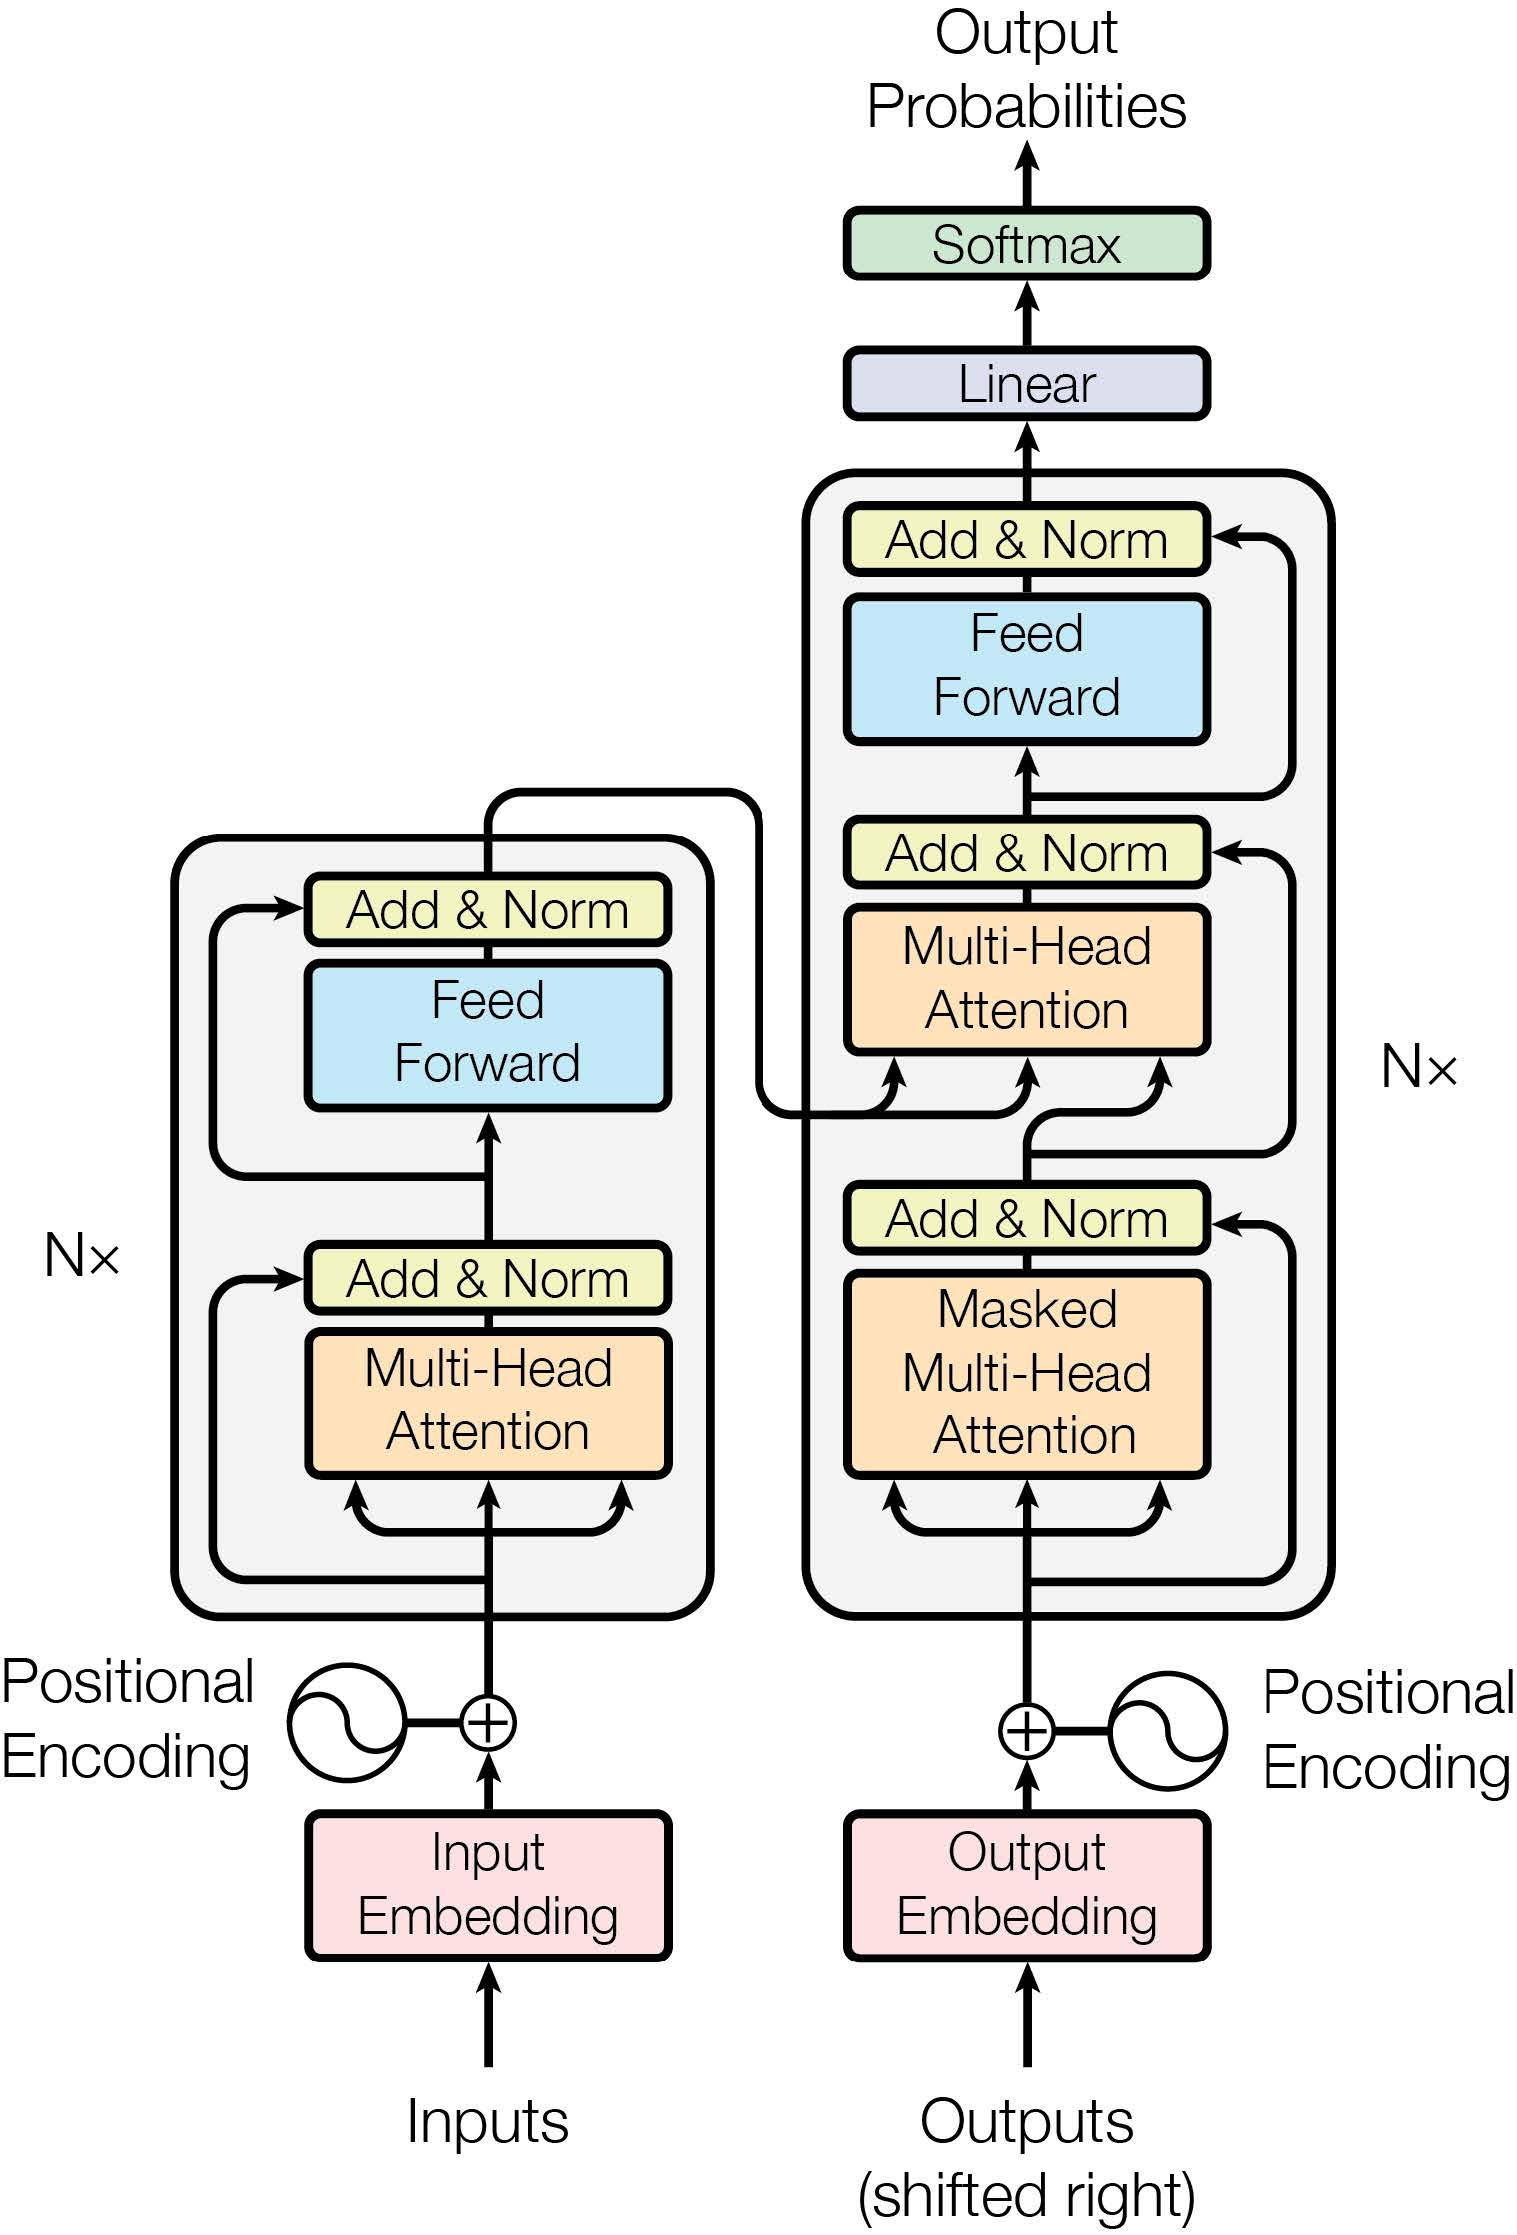
\includegraphics[width=0.45\linewidth]{img/transformer.jpg}          
    \caption{Transformer架构图}
    \label{fig:transformer}
\end{figure}

% \section{改进策略}
\section{改进策略}\label{sec-4}
\subsection{非线性激活函数的选取}\label{sec-4:nonlinear-activation}
本策略来自论文\textit{GLU Variants Improve Transformer}\citep{shazeerGLUVariantsImprove2020}。

Transformer模型通过多头注意力层和FFN层交替工作。FFN层存在于Transformer架构的编码器和解码器部分中。这个网络的结构是:
    $$
    \text{FFN}(x, W_1, W_2, b_1, b_2) = \max(0, xW_1 + b_1)W_2 + b_2
    $$
    其中,$ x $ 是输入,$ W_1 $ 和 $ W_2 $ 是权重矩阵,$ b_1 $ 和 $ b_2 $ 是偏置向量。
    
    这个公式首先通过一个线性变换 $ xW_1 + b_1 $,然后通过 ReLU 激活函数,最后再通过另一个线性变换 $ W_2 $ 和偏置 $ b_2 $。
    
    在本文中,作者对前馈网络进行了一些调整,取消了偏置项。这样做的目的是为了简化模型和提高训练效率。调整后的前馈网络结构是:
    $$
    \text{FFN}_{\text{ReLU}}(x, W_1, W_2) = \max(0, xW_1)W_2
    $$
    这个公式中,去掉了偏置项 $ b_1 $ 和 $ b_2 $,只保留了 ReLU 激活函数和两个权重矩阵。
    
    除了 ReLU 激活函数,还有一些其他的激活函数被用于前馈网络中。例如,基于高斯误差函数的激活函数 GELU 可以用于前馈网络,其结构是:
    $$
    \text{FFN}_{\text{GELU}}(x, W_1, W_2) = \text{GELU}(xW_1)W_2
    $$
    GELU 激活函数可以更好地模拟神经网络的随机正则化行为,从而提高模型的性能。
    
    另一个被用于前馈网络的激活函数是 Swish。Swish 激活函数是一个自门控的激活函数,它可以自动调节每个神经元的输出。基于 Swish 激活函数的前馈网络结构是:
    $$
    \text{FFN}_{\text{Swish}}(x, W_1, W_2) = \text{Swish}(xW_1)W_2
    $$
    Swish 激活函数在某些情况下可以提高神经网络的性能,因此在设计前馈网络时,可以根据具体的应用场景选择合适的激活函数。
\subsubsection{门控线性单元(GLU)及其变种}
    在神经网络中,门控线性单元(GLU)作为一种有效的激活机制被广泛应用。其核心思想是通过引入一个门控机制来调节信息流动,从而增强模型的表达能力。GLU 的数学表达式为:
    $$
    \text{GLU}(x, W, V, b, c) = \sigma(xW + b) \otimes (xV + c)
    $$
    这里,$ x $ 表示输入向量,$ W $ 和 $ V $ 是权重矩阵,而 $ b $ 和 $ c $ 分别是偏置项。符号 $ \sigma $ 表示sigmoid激活函数,$ \otimes $ 表示逐元素乘法。
    
    进一步简化 GLU 模型,如果去掉激活函数 $ \sigma $,则得到一种称为 Bilinear 的变体,其公式为:
    $$
    \text{Bilinear}(x, W, V, b, c) = (xW + b) \otimes (xV + c)
    $$
    
    在此基础上,研究者们提出了几种基于不同激活函数的 GLU 变体,以探索更优的性能表现:
    \begin{itemize}
    	\item \textbf{ReGLU}:使用ReLU激活函数替代sigmoid:
    	$$
    	\text{ReGLU}(x, W, V, b, c) = \max(0, xW + b) \otimes (xV + c)
    	$$
    	
    	\item \textbf{GEGLU}:则采用GELU作为激活函数:
    	$$
    	\text{GEGLU}(x, W, V, b, c) = \text{GELU}(xW + b) \otimes (xV + c)
    	$$
    	
    	\item \textbf{SwiGLU}:引入了参数化的 Swish 激活函数,其中 $ \beta $ 是可学习的参数:
    	$$
    	\text{SwiGLU}(x, W, V, b, c, \beta) = \text{Swish}_\beta(xW + b) \otimes (xV + c)
    	$$
    \end{itemize}
    
    接下来,我们考虑将上述激活函数应用于前馈神经网络(FFN),构建了一系列新的 FFN 结构:
    $$
    \text{FFN}_{\text{GLU}}(x, W, V, W_2) = (\sigma(xW) \otimes xV) W_2
    $$
    $$
    \text{FFN}_{\text{Bilinear}}(x, W, V, W_2) = (xW \otimes xV) W_2
    $$
    $$
    \text{FFN}_{\text{ReGLU}}(x, W, V, W_2) = (\max(0, xW) \otimes xV) W_2
    $$
    $$
    \text{FFN}_{\text{GEGLU}}(x, W, V, W_2) = (\text{GELU}(xW) \otimes xV) W_2
    $$
    $$
    \text{FFN}_{\text{SwiGLU}}(x, W, V, W_2) = (\text{Swish}_1(xW) \otimes xV) W_2
    $$
\subsubsection{模型评估}
\noindent\textbf{翻译任务实验}

    作者使用基于Transformer架构的T5模型在文本翻译任务上进行实验,比较了不同激活函数变体在65,536次和524,288次训练步骤后的log-perplexity表现。
    
    实验结果表\ref{tab:results}表明,GEGLU和SwiGLU变体在这两个训练阶段都取得了最低的困惑度(perplexity),这说明它们在提高翻译质量方面具有显著的优势。
    
    
\noindent\textbf{语言理解任务实验}

    为了进一步验证这些变体的有效性,作者在GLUE(General Language Understanding Evaluation)基准测试上进行了实验。
    
    结果表\ref{tab:glue_results1}显示,在多个子任务中,SwiGLU、ReGLU 和 Bilinear 变体均表现出色,至少在三个不同的任务上达到了最优或接近最优的结果。这一发现证明了这些变体在语言理解任务中的有效性。
    
    此外,作者还探讨了使用预训练模型进行去噪,并随后在下游任务中应用不同激活函数的效果。
    
    实验表\ref{tab:glue_results2}表明,在基于预训练-微调的语言理解任务中,GEGLU、Bilinear 和 SwiGLU 变体同样展示了优异的表现,分别在多个任务上取得了最佳成绩。这些结果支持了假设,即这些激活函数变体不仅能增强模型的表现力,还能促进模型从大规模预训练数据中更有效地迁移知识到特定任务中。
    
    
    综合以上实验结果,作者提出相应建议:
    \begin{itemize}
    	\item \textbf{翻译任务:}鉴于GEGLU和SwiGLU在翻译任务上的出色表现,我们推荐在未来的翻译模型设计中优先考虑这两种激活函数变体。
    	\item \textbf{语言理解任务:}对于语言理解任务,尤其是涉及复杂语义分析的任务,SwiGUE、ReGLUE 和 Bilinear 是值得尝试的选择,因为它们能够提供更好的表达能力和泛化性能。
    	\item \textbf{预训练-微调框架:}在采用预训练-微调框架处理语言理解任务时,GEGLU、Bilinear 和 SwiGLU 的组合可能是提升模型性能的有效策略。
    \end{itemize}
\subsection{LN结构调整}\label{sec-4:ln-adjust}
本策略来自论文\textit{On Layer Normalization in the Transformer Architecture}\citep{xiongLayerNormalizationTransformer2020}。

该文研究了Transformer架构中层归一化(Layer Normalization)的位置对模型训练稳定性的影响,一共进行了三次实验。在传统的Transformer中,层归一化位于残差块之间(称其为Post-LN),这会导致在初始化时输出层附近的参数梯度较大。使用较大的学习率会导致训练不稳定。如图\ref{fig:layer-structure}.

\begin{figure}[ht]
    \centering
    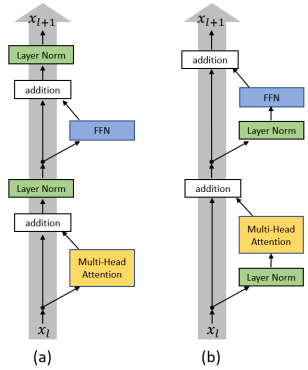
\includegraphics[height=7cm]{img/LN/LN-1.jpg}
    \caption{(a) Post-LN Transformer layer; (b) Pre-LN Transformer layer.}
    \label{fig:layer-structure}
\end{figure}

同时为了验证其性能,该文同时验证了学习率预热阶段的依赖性:为了稳定训练,通常需要一个精心设计的学习率预热阶段。这个阶段虽然对最终性能至关重要,但会减慢优化过程并增加超参数调整的复杂性。以上为该文的两个主要贡献。

\subsubsection{warm-up机制}

首先我们需要了解什么是warm-up。在优化Transformer结构时,除了像训练一般模型一样设置初始学习率与它的衰减策略(Adam,SGD),往往还需要在训练的初始阶段设置一个非常小(接近0)的学习率,让它经过一定的迭代轮数后逐渐增长到初始的学习率,这个过程也被称作warm-up阶段。

warm-up是原始Transformer结构优化时的一个必备学习率调整策略。Transformer结构对于warm-up的超参数(持续轮数、增长方式、初始学习率等)非常敏感,若调整不慎,往往会使得模型无法正常收敛。

该文在IWSLT14 De-En翻译数据集上使用Transformer模型对warm-up的效果进行验证,采用Adam和SGD两种随机优化器,分别测试了两种学习率($1 \times 10^{-3}$, $5 \times 10^{-4}$)在没有warm-up(0轮), warm-up迭代轮数不足(500轮)和迭代轮数充足(4000轮)情况下模型的验证集Loss与BLEU分数,结果如图\ref{fig:performance}所示。

\begin{figure}[ht]
    \centering
    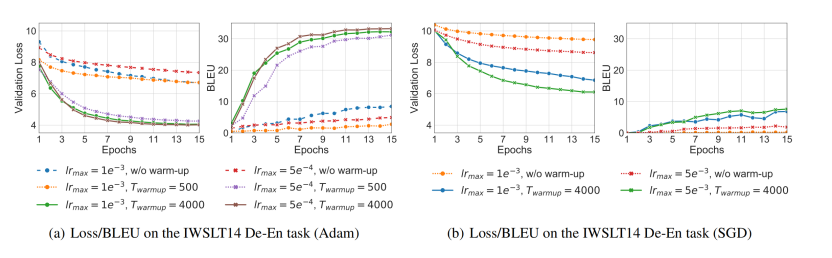
\includegraphics[width=\textwidth]{img/LN/LN-2.jpg}
    \caption{Performances of the models optimized by Adam and SGD on the IWSLT14 De-En task.}
    \label{fig:performance}
\end{figure}

从实验中可以看出,模型最终性能对无论是warm-up所需迭代轮数还是学习率的大小都非常敏感,由于Transformer优化困难的阶段是在训练的初始阶段,warm-up也只是在迭代的前若干轮起作用,因此从模型的初始化阶段开始探究原因。

\subsubsection{LN执行对对梯度范数的影响}

Transformer层的初始化方式通常是Xavier方法,通过对各隐层梯度值进行分析可以证明,在初始化点附近的Post-LN Transformer结构最后一层的梯度值非常大,同时随着反向传播的前传会导致梯度值迅速衰减。这种在各层之间不稳定的梯度分布必然会影响优化器的收敛效果,导致训练过程初始阶段的不稳定。造成Post-LN Transformer梯度分布出现问题的核心原因在于各子层之后的Layer Normalization层会使得各层的输入尺度与层数\(L\)无关,因此当Layer Normalization对梯度进行归一化时,也与层数\(L\)无关。

作者提出Pre-LN Transformer,即将层归一化放在残差块内部,在每个子层(如自注意力机制或前馈神经网络)之后进行归一化,而不是在残差连接之后,并且在整个网络最后输出之前也增加一个Layer Normalization层来对梯度进行归一化。

使用相同的方法对Pre-LN Transformer结构进行分析后,发现最后一层Layer Normalization层的输入尺寸的量级只有Post-LN的\(\sqrt{1/L}\)倍,并且每个LN层都会对梯度以\(\sqrt{L}\)的比例归一化。所以对于Pre-LN结构来说,其每层梯度范数都近似不变。

该文在IWSLT 14 De-En数据集对两种结构在初始化附近以及经过了warm-up阶段的梯度范数进行了实验验证,结果如图\ref{fig:gradients}所示。
\begin{figure}[h]
    \centering
    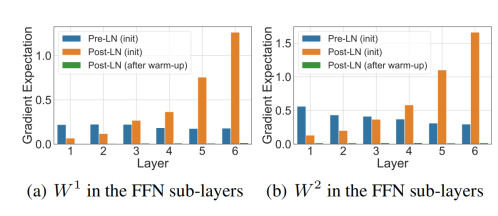
\includegraphics[width=11cm]{img/LN/LN-3.jpg}
    \caption{The norm of gradients of different layers in the Transformer.}
    \label{fig:gradients}
\end{figure}

可以看出,相比于Post-LN结构梯度分布的不稳定,Pre-LN在各层之间梯度范数几乎保持不变,这种结构明显更利于优化器进行优化。而在进行一定轮数的warm-up后,Post-LN的梯度范数也基本保持不变,并且其量级非常小,这也验证了理论。

\subsubsection{模型评估}

最后,在IWSLT、WMT和BERT三个任务上实验验证了是否可以在Pre-LN结构中去掉warm-up,结果如图\ref{fig:iwslt-wmt5}、\ref{fig:bert}所示。
\begin{figure}[h]
    \centering
    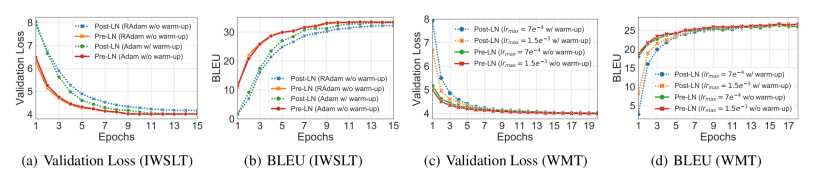
\includegraphics[width=\textwidth]{img/LN/LN-4.jpg}
    \caption{Performances of the models on the IWSLT14 De-En task and WMT14 En-De task.}
    \label{fig:iwslt-wmt5}
\end{figure}

\begin{figure}[ht]
    \centering
    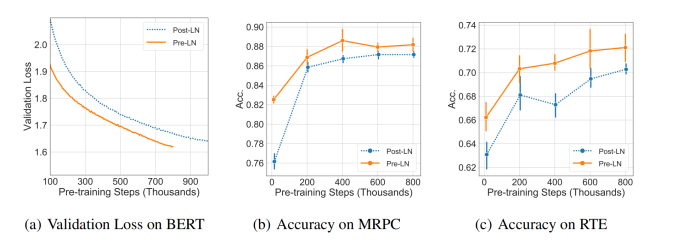
\includegraphics[width=14cm]{img/LN/LN-5.jpg}
    \caption{Performances of the models on unsupervised pre-training (BERT) and downstream tasks.}
    \label{fig:bert}
\end{figure}

实验结果表明,当使用Pre-LN结构时,warm-up阶段已经不再是必需,并且Pre-LN结构可以大幅提升Transformer的收敛速度。对于机器翻译任务(IWSLT/WMT),不需要warm-up的Pre-LN结构可以比Post-LN收敛快1倍左右,而在BERT上,Pre-LN在下游任务上达到和Post-LN相同的性能也只需要后者迭代轮数的1/3左右,并且最终的效果也更好。

总之,Pre-LN Transformer在没有学习率预热阶段的情况下,可以在多种应用中达到与Baseline相当的结果,同时显著减少了训练时间和超参数调整。

\subsection{相对位置编码}\label{sec-4:rel-pos-encoding}
本策略来自论文\textit{Self-Attention with Relative Position Representations}\citep{shawSelfAttentionRelativePosition2018}。

Transformer的架构Self-Attention机制本质上是无序的,即它对输入序列的排列顺序不敏感,这导致原始Transformer模型难以直接捕捉到token之间的相对或绝对位置信息。为了解决这个问题,通常的做法是在输入嵌入中加入位置编码(Positional Encoding),以此间接地向模型提供序列元素的位置信息。

本文提出了一种方法,通过改进Self-Attention机制,在其内部直接整合token间的相对位置关系向量,从而打破了原有的排列不变性,使得Self-Attention不仅能够感知到序列中元素的位置,而且更高效地编码这些位置信息,无需依赖外部附加的位置特征。
\subsubsection{关系感知自注意力机制}
考虑一个有向全连接图,其节点由输入元素构成,并且每条从$x_i$指向$x_j$的边都附带有一对向量$\alpha_{ij}^V, \alpha_{ij}^K \in \mathbb{R}^{d_\alpha}$作为特征描述,这里$d_a = d_z$。这些向量在所有注意力头中共享,以捕捉节点间的相对位置信息。通过引入边的特性表示,传统的自我注意(Self-Attention)机制被重新定义为如下形式:
\begin{align*}
    z_i &= \sum_{j=1}^{n} \alpha_{ij} \left( x_j W^V + \alpha_{ij}^V \right)\\
    \alpha_{ij} &= \frac{\exp e_{ij}}{\overunderset{n}{k=1}{\sum}\exp e_{ik}}\\
    e_{ij} &= \frac{x_i W^Q \left( x_j W^K + \alpha_{ij}^K \right)^T}{\sqrt{d_z}}
\end{align*}
其中,每个Value ($T^V$) 和 Key ($T^K$) 都附加了位置关系编码,从而使得该注意机制不再对节点顺序保持不变。
\subsubsection{相对位置编码}
鉴于计算复杂度、内存占用以及远距离精确位置信息的边际效益递减等因素,本文中对相对位置距离施加了最大限制$k$。具体而言,当节点间的实际距离超出这一界限时,我们将它们的位置差异截断至这一范围内。这可以形式化为:
\begin{align*}
    a_{ij}^K &= w_{\text{clip}(j-i, k)}^K\\
    a_{ij}^V &= w_{\text{clip}(j-i, k)}^V\\
    \text{clip}(x, k) &= \max(-k, \min(k, x))
\end{align*}
其中,$\text{clip}$函数确保任何一对节点之间的相对位置编码不会超过预设的最大距离$k$。在这种情况下,模型只需要学习有限集合的参数:对于Key ($\omega^K = (\omega_{-k}^K, \ldots, \omega_k^K)$) 和 Value ($\omega^V = (\omega_{-k}^V, \ldots, \omega_k^V)$),每个方向各有$k$个不同的位置权重。
\subsubsection{高效实现}
引入相对位置编码后,作者将原本的键值$k_{ij}$分解成两个独立的部分,以便分别进行高效的矩阵运算。这使得每个部分都可以通过并行计算加速,具体公式如下:
$$
e_{ij} = \frac{x_i W^Q \left( x_j W^K \right)^T + x_i W^Q \left( a_{ij}^K \right)^T}{\sqrt{d_z}}
$$
其中,第一项与未添加相对位置编码时的计算方法相同,而第二项则利用了位置编码$b_{ij}^K$进行了调整。设上式右侧为$e'_{ij}$,令$x_i W^Q = q_i$,并且$a_{ij}^K = k_{ij}$,忽略分母,则有$e'_{ij} = q_i k_{ij}^T$。

在这样的设置下:
\begin{itemize}
\item 我们拥有$bh \times n$个$q_i$,每个$q_i$的维度是$d_z$。
\item 同样地,存在$n \times n$个$k_{ij}$,每个$k_{ij}$的维度也是$d_z$。
\end{itemize}

为了实现高效矩阵运算,需要对$q_i$和$k_{ij}$进行重新组织:
\begin{itemize}
\item $q_i$可以被视作$n \times bh$个$q'_i$,每个$q'_i$仍具有$d_z$的维度。
\item 对于$k_{ij}$,它同样可以被看作$n \times n$个$k'_{ij}$,每个$k'_{ij}$保持$d_z$的维度不变。
\end{itemize}

这样一来,我们可以针对$q'_i$和$k'_{ij}$执行$n$次并行的矩阵乘法操作,每次涉及两个大小分别为$bh \times d_z$和$d_z \times n$的矩阵。完成这些计算之后,再将结果重新组织回原来的形状,以完成$e_{ij}$两部分的高效并行化计算。

此时我们便可以对$q'_i$和$k'_{ij}$进行$n$个并行化的两个大小为$bh \times d_z$和$d_z \times n$的矩阵计算来加速计算。最终再重新reshape回原始的大小即可完成$e_{ij}$两个部分的高效并行化计算。
\subsubsection{模型评估}
本篇论文主要是用于NLP领域,使用newstest2014测试集,WMT 2014英语到德语(EN-DE)和英语到法语(EN-FR)翻译任务,其实验结果如表\ref{tab:results1},\ref{tab:clipping-distance-results},\ref{tab:ablation-results}。

总的来说,本文提出了一种扩展自注意力机制的方法,该方法能够有效地将序列元素间的相对位置信息融入到模型中,从而提升了机器翻译任务的性能。通过这种改进,模型可以在不依赖显式的位置编码(即硬位置编码)的情况下处理位置信息。

不过论文中并未直接对比新方法与传统硬位置编码在效果上的差异。


\subsection{稀疏注意力机制}\label{sec-4:sparse-attention}
本策略来自论文\textit{Generating Long Sequences with Sparse Transformers}\citep{childGeneratingLongSequences2019}。

Transformer最被诟病的一个问题是它的时间复杂度以及空间复杂度和输入序列的长度成二次方的关系$O(n^2)$。而这篇文章提出的Sparse Transformer方法使用稀疏自注意力替代了传统Transformer的密集自注意力,将Transformer的复杂度降低到$O(n^{3/2})$。

在CIFAR-10数据集上,使用一个128层的自注意力模型。对注意力进行可视化,得到图\ref{fig:iwslt-wmt1}:

\begin{figure}[h]
    \centering
    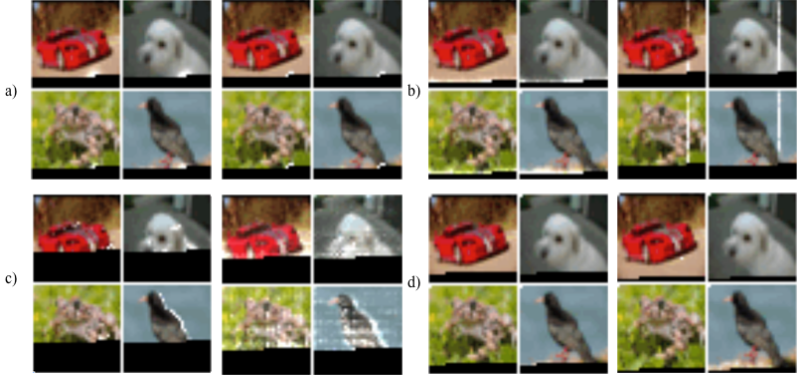
\includegraphics[width=\textwidth]{img/SC/SC1.jpg}
    \caption{Learned attention patterns from a 128-layer network on CIFAR-10 trained with full attention.}
    \label{fig:iwslt-wmt1}
\end{figure}

白色区域是注意力机制的高权值位置,黑色区域是被mask掉的位置,从a到d为层数逐渐加深的过程,可以看到注意力头的权重分布从浅至深呈现出“周围——行列——全局——全局稀疏”的变化过程。那么直接在注意力头上利用这种稀疏性是否可以加速计算,这需要一系列设计和验证。

\subsubsection{连接模式}

像GPT这样的自回归模型,使用的是之前所有时间片的内容来预测当前时间片的结果。传统的Transformer需要为之前的所有时间片计算一个权值,所以传统Transformer的自注意力机制的复杂度是$O(n^2)$。如下图\ref{fig:iwslt-wmt2}(a)中为大小$6\times6$图像的注意力和长度为16的注意力连接矩阵。

\begin{figure}[h]
    \centering
    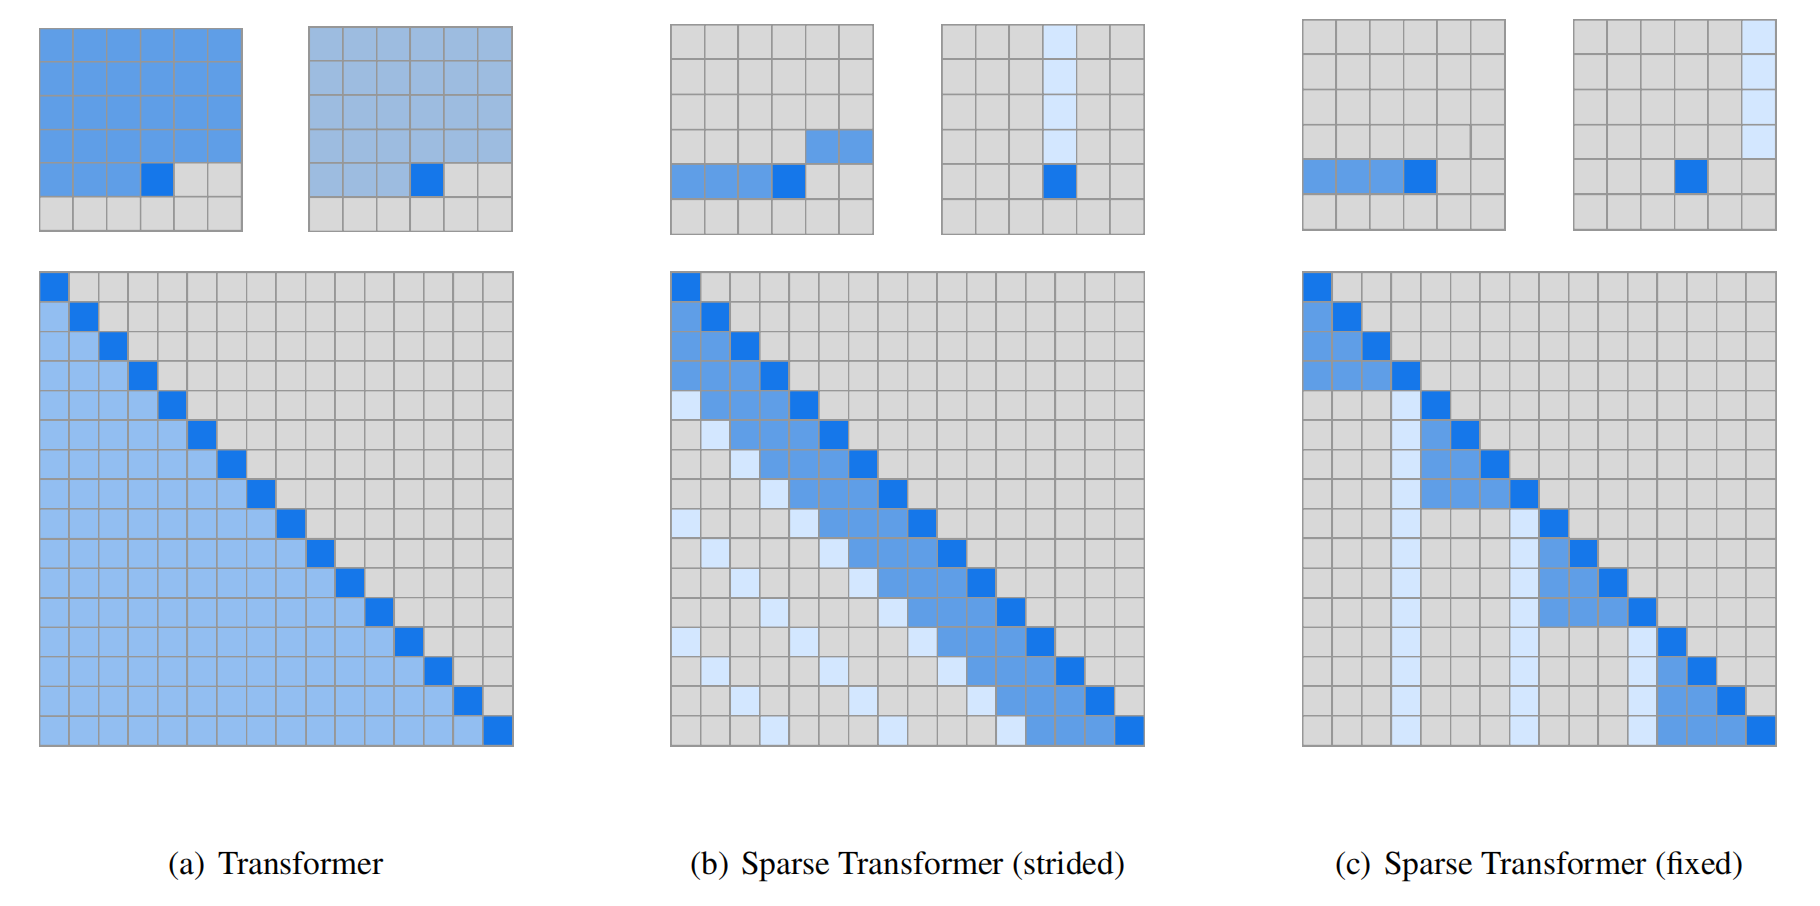
\includegraphics[width=\textwidth]{img/SC/SC2.jpg}
    \caption{Two 2d factorized attention schemes we evaluated in comparison to the full attention of a standard Transformer (a).}
    \label{fig:iwslt-wmt2}
\end{figure}

传统的自注意力的计算方式可以表示为:
\[
\text{Attention}(Q, K, V) = \text{softmax}\left(\frac{QK^T}{\sqrt{d_k}}\right)V
\]

该计算方式复杂度最高的地方是$QK^T$,而Sparse Transformer的核心是只让设置好的像素点参与自注意力的计算。这里不是只选取设置好位置上的像素点,其他mask掉,因为这样并不能降低模型的复杂度。

为了实现上述目标,我们这里引入一个名为连接模式(Connectivity Pattern)的变量,它表示为$S = \{S_1, S_2, \ldots, S_n\}$,其中$S_i$表示预测第$i$个时间片的索引。形象地说,它可以表示为一个由0和1组成的二维矩阵,二维矩阵中的数值为1表示该位置的像素点参与自注意力的计算。如在上图中,位置为28,则传统自注意力中$6\times6$大小$S_{28}$的表示为(a)的上半部分,其中深色部分为1,浅色部分为0。

在Sparse Transformer的自注意力计算中,连接模式只作用在$K$和$V$的计算上,计算过程如下所示。

1. 对于第 \(i\) 个时间片的输入,首先使用 \( \text{key} \) 和 \( \text{value} \) 的权值矩阵乘以输入特征,得到 \( K \) 和 \( V \)。然后再将连接模式 \( S_i \) 作用到 \( K \) 和 \( V \) 上,得到稀疏的特征 \( K_{S_i} \) 和 \( V_{S_i} \)。
   \[
   K_{S_i} = (W_k x_j)_{j \in S_i}, \quad V_{S_i} = (W_v x_j)_{j \in S_i}
   \]

2. 然后使用稀疏特征得到第 \(i\) 个时间片的自注意力结果。
   \[
   a(x_i, S_i) = \text{softmax}\left(\frac{(W_q x_i) K_{S_i}^T}{\sqrt{d}}\right) V_{S_i}
   \]

3. 最后再将 \(n\) 个时间片的结果合并起来,得到最终的结果。
   \[
   \text{Attend}(X, S) = (a(x_i, S_i))_{i \in \{1, \ldots, n\}}
   \]

其中 \( W_q \),\( W_k \) 以及 \( W_v \) 分别是 \( \text{Query} \),\( \text{Key} \),\( \text{Value} \) 三个向量对应的权值矩阵。Sparse Transformer 通过让连接模式作用到 \( K^T \) 上,从而降低了 \( QK^T \) 的复杂度。

我们这里已经定义好了稀疏自注意力机制的通用计算方式,接下来要做的就是设计不同的连接模式。对于每个自注意力的计算,我们可以使用若干不同的注意力核。在论文中,作者使用了2个注意力核(行+列),也可以扩展到更高的维度。

\subsubsection{注意力核}

Strided Attention由两种形式的连接模式组成,如上图\ref{fig:iwslt-wmt2}(b)所示,其包含行和列两种注意力核。假设步长为 \( l \),行注意力核指的是在连接模式中,当前时间片的前 \( l \) 个时间片的值是1,其余的值是0。列注意力核指的是连接模式中每隔 \( l \) 个时间片的值为1,其余值为0。

行注意力核和列注意力核的表达式如下:
\begin{align*}
A_i^{(1)} &= \{t, t+1, \ldots, i\}, \quad t = \max(0, i-l) \\
A_i^{(2)} &= \{j: (i-j) \mod l = 0\}
\end{align*}

对于图片生成这一类任务来说,\( l \) 一般为图像的宽或者高。所以复杂度为 \( O(l) = O(\sqrt{n}) \)。

Fixed Attention同样也是由行注意力核和列注意力核组成,如上图\ref{fig:iwslt-wmt2}中(c)所示。行注意力核是当前时间片同行的时间片。表示为下面的式子:
\[
A_i^{(1)} = \{j: (\lfloor j/ l \rfloor = \lfloor i/ l \rfloor)\}
\]

列注意力核表示为:
\[
A_i^{(2)} = \{j: j \mod l \in \{t, t+1, \ldots, l\}\}
\]

其中 \( t = l - c \),Fixed Attention的列注意力核又被叫做滑窗注意力核,超参数 \( c \) 相当于滑窗卷积窗口的大小。上述两个注意力核的复杂度同样为 \( O(\sqrt{n}) \)。

\subsubsection{融入网络}

上面介绍了多种不同形式的注意力核,下面将介绍如何将这些不同形式的注意力核融入到网络中。

传统的Transformer通过如下方式计算注意力核:
\[
\text{attention}(X) = W_p \cdot \text{attend}(X, S)
\]
其中 \( W_p \) 表示后注意力权重矩阵。本文作者提出了以下三种新的方式:

1. 每个残差块使用不同的注意力核类型,一个深层网络是由多个连续的残差块组成的,对于每个残差块,我们可以使用不同类型的注意力核,表示为下式:
\[
\text{attention}(X) = W_p \cdot \text{attend}\left(X, A^{(r \mod p)}\right)
\]
这里 \( r \) 是当前残差块的索引,\( p \) 是分解注意力头的数量。

2. 第二个方式是每个注意力头都计算所有类型的注意力核,然后合并他们的结果,如下式所示:
\[
\text{attention}(X) = W_p \cdot \text{attend}\left(X, \bigcup_{m=1}^p A^{(m)}\right)
\]

3. 第三个方式是对于多头的注意力机制,每组头选择一个形式的注意力核,然后将他们合并起来,如下式所示:
\[
\text{attention}(X) = W_p \left(\text{attend}(X, A^{(i)})\right)_{i \in \{1, \ldots, n_h\}}
\]

其中 \( n_h \) 组不同的注意力核会并行计算,然后在特征维度进行特征拼接。实验结果证明这种方式是最好的融合策略。


\subsubsection{模型评估}
通过在包括自然图像、文本和原始音频的密度建模任务上的经验测试来验证架构,结果总结见表\ref{tab:performance_comparison},\ref{tab:model_comparison}。可以发现,除了运行速度明显快于全注意力模型外,稀疏模式还收敛到更低的误差。这可能表明引入的稀疏模式具有有用的归纳偏好,或者全注意力存在潜在的优化问题。
% \section{模型构建}
\section{简易Transformer模型的构建过程}\label{sec-5}

本节主要介绍如何构建简易的Transformer模型。需要注意的是,本节的重点在于介绍我们自定义的Transformer及各个模块,因此对于如何调用数据集和训练模型没有做过多的阐释。在下一节中,我们将重点介绍如何利用更复杂更多样的数据集进行模型训练以及如何通过选择不同数据集写出不同风格和类型的诗词。

在本项目中,我们试图只使用Pytorch库中的线性层等简单的模块,自己实现Transformer的相应机制和模块,构建一个能够根据输入的前半句古诗输出后续内容的Transformer。

在实现上,我参考了kaggle上\href{https://www.kaggle.com/code/alionsss/pytorch-transformer-x/notebook}{PyTorch示例——使用Transformer写古诗}的项目架构,挪用了其数据集、编码器、位置编码的实现和整体框架。

\texttt{./simpleTransformer/classes.py }中提供了所有类定义的实现(包含上述数据集和编码器);\texttt{./simpleTransformer/trans.ipynb}中提供了整个模型的全流程实现。

\subsection{模块类型的定义}

下面我们逐模块的介绍我们的自定义类。

\subsubsection{关于批次的处理}

在第\ref{sec-3}节中,我们并未关注到批次的相关信息。但在实际训练中,通常会使用多批次训练的方法,使得更加有效的利用现有计算资源,提高计算效率和收敛效果。因此我们需要使得构建的模块能够适用于多批次的训练。幸运的是,Pytorch提供了Dataloader处理批次数据,但仍然需要注意在计算损失函数、提供掩码时,需要根据实际情况将张量变形或扩展成相应的具有batch\_size的形状。

在后续内容中,如无特别说明,不再叙述处理批次导致的形状变化。

\subsubsection{嵌入层}

嵌入层主要用于将一个序列转化为编码器、解码器的输入,请关注\texttt{./simpleTransformer/classes.py}中的Embedding类。

具体来讲,对于一个序列长度为$s$,词典大小为$v$的形状为$(s,)$的序列输入,每个位置的值代表一个汉字,我们首先将其转化为形状为$(s,v)$的独热向量,再经过线性层$(v,h)$,得到形状为$(s,h)$的嵌入向量。

\subsubsection{注意力模块}

请关注\texttt{./simpleTransformer/classes.py}中的Attention类。

自注意力和交叉注意力机制的逻辑实质上是相同的,只是在调用时需要使用不同的输入参数。因为本项目中只会使用到自注意力和交叉注意力机制,因此我们假定要么$q,k,v$的输入相同,要么$k,v$的输入相同。

具体实现中,首先我们需要考虑如何实现多头注意力机制。如果我们将数据分别训练$a$次,再将结果拼接在一起,实现复杂度上比较高。

通过探索发现,我们可以将所有$a$个头的$W_Q^i,W_K^i,W_V^i$拼接在一起,使用和单头注意力机制相同的逻辑计算$Q,K,V$,以$Q_i$为例
$$
[Q_1, Q_2,\cdots , Q_a] = [XW_Q^1 , XW_Q^2 , \cdots, XW_Q^a ] = X[W_Q^1, W_Q^2, \cdots, W_Q^a],
$$
这样在代码实现上更加简洁和高效。

之后通过Pytorch提供的view()/permute()/transpose()/expand()等方法,\textbf{将注意力头数作为单独的维度提取出来},再使用矩阵乘法等算子计算即可。

这也体现了在底层实现上基础算子的可扩展性,以矩阵乘法为例,其默认行为是计算输入的后两个维度的矩阵乘积,这使得能够计算更多维的张量的矩阵乘积。

另一点想要额外说明的是,\textbf{注意力机制不要求$q,k,v$\footnote{用小写字母代表原始输入而非经过$W_Q,W_K,W_V$变换后得到的$Q,K,V$。}的维数相等},交叉注意力机制中编码器输出$X:(src_s,h)$和解码器输入$Y:(tgt_s,h)$的维数也可以不相同,仍然可以进行注意力的计算:
\begin{align*}
    Q &=X W_Q , \ &(tgt_s,h) = (tgt_s, h) \times (h,h) \\
    K &=X W_Q , \ &(src_s,h) = (src_s, h) \times (h,h) \\
    V &=X W_Q , \ &(src_s,h) = (src_s, h) \times (h,h) \\
    Z &= \text{softmax}(\frac{QK^T}{\sqrt{h}}) V, \ &(tgt_s, h) = (tgt_s, h) \times (h, src_s) \times (src_s, h),
\end{align*}
此时我们的注意力输出$Z$仍然和需要迭代计算的编码器输入$Y$维度相同,因此能够进行若干层解码器的计算。


\subsubsection{掩码}

请关注\texttt{./simpleTransformer/classes.py}中的Transformer类中关于mask的部分,部分实现如图\ref{fig:simpletT-mask}。

\begin{figure}[h]
    \centering
    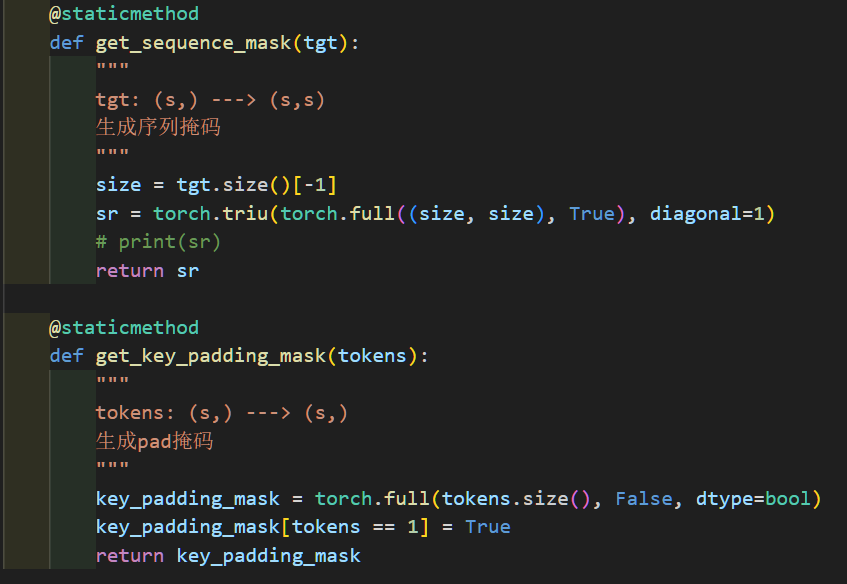
\includegraphics[width=0.8\linewidth]{img/simpleT/simpleT-mask.png}
    \caption{两种掩码的实现}
    \label{fig:simpletT-mask}
\end{figure}

由于我们使用了批量训练,同一批次的数据的序列长度可能不同,但在训练过程中我们将这一个参数进行了固定,因此我们需要调整数据使得同一批次的数据的序列长度相同。

我们采取在数据末尾填充相应的“PAD”符号作为填充占位符来解决这一问题。但这会引发又一个问题,模型可能将“PAD”作为出现频次较高的字符进行学习,进而导致预测输出中大量输出“PAD”。为此,我们需要把模型的注意力从“PAD”上面拿走。这里“拿走”的行为和在遮蔽未来信息的行为是一致的,在实现上,只需在计算softmax之前将这些位置上置$-\infty$,计算出来的结果这些位置上就会是$0$。

此外我们还需要实现在\label{sec-2:mask}中提到的针对解码器自注意力输入的掩码。另外,在实现过程中我还思考了交叉注意力为什么不需要遮蔽未来信息:在交叉注意力中,查询(Query)来自解码器的当前状态,而键(Key)和值(Value)来自编码器的输出。编码器的输出是已经处理好的特征向量,这些特征向量之间没有时间顺序的依赖关系,而查询Q相互之间是“独立的”,因此交叉注意力不需要防止未来信息的泄露。

\subsubsection{TransformerEncoderDecoder模块}

请关注\texttt{./simpleTransformer/classes.py}中的TransformerEncoderDecoder类。

在这里,我们实现了Transformer模型的主要模块,提供自定义编码器、解码器的层数,注意力的头数,掩码,前馈神经网络隐层维度等。

在这里需要关注的是,交叉注意力机制中,解码器的输入(也就是交叉注意力机制的$k,v$)来自于解码器输出的最后一层,而非每个解码器层的输出。这进一步表明,解码器和编码器在Transformer架构中是两个相对独立的结构。

\subsubsection{其他}

\paragraph{残差连接}

这里的实现和原理比较简单,残差连接的具体实现在TransformerEncoderDecoder类中,这里我们实现了改进策略中Layernorm的结构调整(\ref{sec-4:ln-adjust}),可以在调用时指定norm\_first参数来决定使用哪一种Layernorm,如果\texttt{norm\_first == True},则使用Pre-LN Transformer layer。

\paragraph{层归一化} 请关注\texttt{./simpleTransformer/classes.py}中的LayerNorm类。在此我们只关注一个点,在实现层归一化时,不应假定矩阵的维数,而是直接将其最后一层归一化即可,这样提高了我们代码的可复用性和可扩展性。

\paragraph{全连接前馈神经网络} 请关注\texttt{./simpleTransformer/classes.py}中的FeedForward类。这里我们提供了两种可选的激活函数,部分实现了\ref{sec-4:nonlinear-activation}中的改进策略,分别是RELU和GELU。
\\

除了以上类外,还有一些较为简单的类,比如位置编码(PositionalEncoding类)、预测层(Prediction类)等,不再赘述。

\paragraph{模型构建} 请关注\texttt{./simpleTransformer/classes.py}中的Transformer类,我们将所有需要的模块分别初始化后,通过前向传播路径拼装到一起,构成最终的Transformer模型。我们还在这个类中为注意力模块添加了默认掩码。

\subsection{模型训练和表现}

将上述模块集成为Transformer后,我们使用./data/poetry.txt中的诗词数据,$\texttt{batch\_size} = 64$, 编码器和解码器层数为$3$,注意力头数$a=4$,迭代$\texttt{epoch} = 50$轮,采取交叉熵损失,进行训练和预测。每轮的损失函数如图\ref{fig:simpleT-loss},预测效果如图\ref{fig:simpleT-performance}。
\begin{figure}[h]
    \centering
    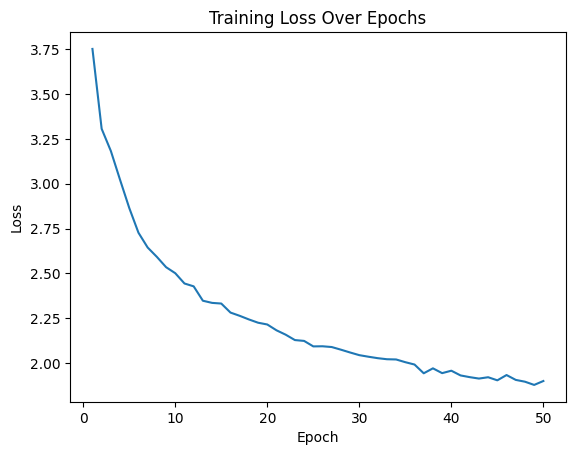
\includegraphics[width = 0.55\textwidth]{img/simpleT/simpleT-loss.png}
    \caption{损失函数变化}
    \label{fig:simpleT-loss}
\end{figure}

\begin{figure}[h]
    \centering
    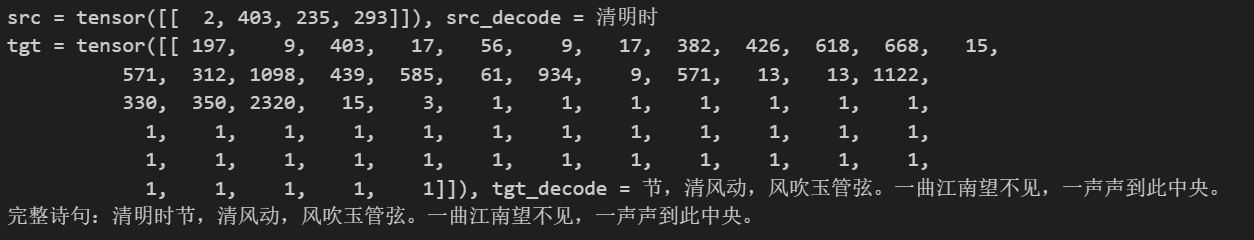
\includegraphics[width = \textwidth]{img/simpleT/simpleT-performance.png}
    \caption{模型预测表现}
    \label{fig:simpleT-performance}
\end{figure}

如希望进行类似测试,可以在\texttt{./simpleTransformer/trans.ipynb}中运行“模型训练”上方所有单元格(类定义和超参数)及“存储模型”(绘制损失函数之后)下方所有单元格(加载模型参数和预测),即可在避免训练的情况下进行相应测试。

\subsection{构建过程中的问题和解决}

在构建模块中,遇到了若干问题,虽然Transformer的架构和注意力机制的计算在原理上已经比较熟悉,但实现过程中仍然出现了许多意料不到的场景,这里简要介绍一下。

\subsubsection{如何执行单元测试}

对于简单的函数和类,我们可以通过构造测试样例等检验函数是否实现了相应功能,但对于嵌套和调用结构复杂的类来讲,如何去验证其行为是否相符,困扰了我相当长的一段时间。

在刚写完相应模块的代码时,我的思路是比较我实现的类和Pytorch提供的类在训练过程中的收敛速度,从而判断实现是否正常,不过这种方法虽然能够发现收敛速度有较大差异,但无法定位到具体的模块,实际上仍需要手动检查每个块的内部逻辑。

经过较长时间的试错后,我发现可以\textbf{针对每个模块,提供相同的输入给我的实现和Pytorch的实现,并且在模型初始化后,指定模型的参数相同,避免参数初始化的随机性影响结果,再比较他们的输出是否相同,以此来判断模块是否正常。}在机器学习中,如果像数学证明中验证两个对象是否相等的逻辑,的确很难进行,但这种排除随机性,验证相同输入下输出是否相同的方法反而是有效和易用的。

\texttt{./simpleTransformer/Comparision.ipynb} 实现了上述自定义模块和Pytorch相应模块的检验。

\subsubsection{维度验证}

在课程学习矩阵求导相关知识时,对于矩阵求导是否正确,课程Note中使用维度进行检验,这依然不符合我的直觉,认为这只能提供一个非常基本和低层次的检验。但在这次作业中,我深刻意识到了维度检验这一方法的重要性和实用性。

Pytorch提供的接口能够便捷的改变张量的形状,但与二维矩阵不同的时,考虑到批次和注意力头数的参与,张量的形状往往可能是三维甚至四维的,在这种情况下,简要运算过程中不同变量的维度信息,能够很方便的检验整个运算过程是否符合我们的预期。

我们以注意力模块为例,展示在实现过程中的维度验证(图\ref{fig:simpleT-dimension})。
\begin{figure}[h]
    \centering
    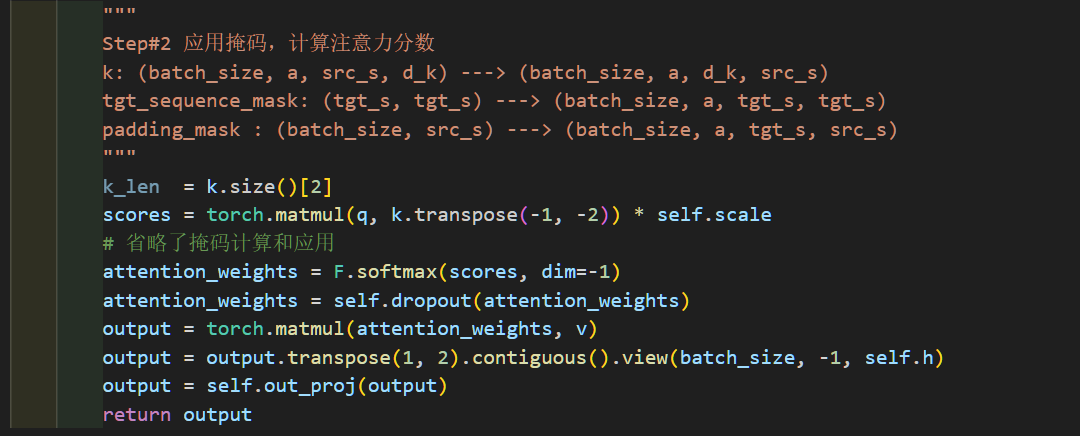
\includegraphics[width=\linewidth]{img/simpleT/simpleT-dimension.png}
    \caption{维度验证在注意力计算中的应用}
    \label{fig:simpleT-dimension}
\end{figure}

\subsubsection{模块的可复用性}

通过类这种面向对象的编程方式,我们能够复用我们定义好的模块。不过python无法导入定义在\texttt{.ipynb}文件中的方法,因此,我们将所有的类定义单独封装在\texttt{./simpleTransformer/classes.py}中,可以通过在其他文件中\texttt{from classes import *}复用我们的类和方法,也方便了后续进行的古诗文写作助手的进一步优化和封装。

另一方面,通过定义多个子模块,我们可以像积木一样任意的拼接各个模块,从而产生不同结构的模型,进行不同的尝试,这也是面向对象编程的一大乐趣。

\subsubsection{如何开发新功能}

如果在现有代码上直接更改,很有可能出现代码无法正常运行,又无法回退的局面。在这次作业中,我尝试带领小组成员一起使用代码版本管理工具,在一定程度上非常有助于开发新功能、扩展新模块,当出现异常时,能够非常简单的回退到原始状态,或进行对比以发现问题所在。不过比较遗憾的是,小组成员并没有太多git使用经验,当模型初步编写完成后和其他两位同学同步开发时,由于需要更新部分接口或操作逻辑,代码版本的不统一造成了一定困难。

这也提示我们,在编写代码时,需要充分考虑到接口的可扩展性,同时理清模型依赖关系,尽可能清晰的完成新功能开发的每一步。
% \section{古诗文写作助手}
\section{古诗文写作助手}\label{sec-7}
\subsection{数据集与预处理}
为了构建一个能够有效生成古典诗词的大语言模型,我们小组选择了来自GitHub上的公开数据集\textit{Chinese-Poetry}作为训练基础。该数据集由同名项目维护,网址为:\url{https://github.com/chinese-poetry/chinese-poetry},涵盖了中国古代文学的广泛领域,包括但不限于诗、词、曲等多种体裁。
    
考虑到模型的特定应用目标——即专注于古诗词的生成——我们在初步的数据收集阶段进行了针对性的选择。具体来说,我们从原始数据集中筛选出了以下几类具有代表性的古诗词条目,以确保数据集的纯净度和相关性:
\begin{itemize}
    \item 曹操诗集:收录了三国时期曹操创作的诗歌作品。
    \item 楚辞:战国时期的楚国诗人屈原等人的抒情长诗。
    \item 纳兰性德:清代著名词人纳兰性德的作品集。
    \item 全唐诗:唐代诗歌的汇总,几乎囊括了所有流传至今的唐诗。
    \item 诗经:中国最早的诗歌总集,包含西周初年至春秋中期的诗歌。
    \item 水墨唐诗:精选唐代诗歌,侧重于描绘自然景观和社会生活。
    \item 宋词:宋代词作的集合,展现了宋朝文人的艺术风采。
    \item 五代诗词:涵盖了五代十国时期的诗歌创作。
    \item 御定全唐诗:清朝康熙年间编纂的官方版唐诗全集。
    \item 元曲:元代戏曲剧本中的唱词部分,体现了当时的文化特色。
\end{itemize}
    
在数据预处理阶段,我们进一步优化了数据结构,以便更好地服务于模型训练的需求。我们的目标是创建一个简洁而易于处理的文本文件(.txt),其中每首古诗词的标题和内容被整合在同一行内,采用“标题:内容”的格式。例如:
\begin{verbatim}
日诗:欲出未出光辣达,千山万山如火发。须臾走向天上来,逐却残星赶却月。
\end{verbatim}

这一过程不仅简化了输入格式,提高了训练效率,还减少了不必要的数据冗余,使得后续的文本处理步骤更为直观易行。最终,经过清理和格式化后的数据被保存为文本文件(.txt),以供模型训练使用。
\subsection{模型训练与封装}
在实现了基本的Transformer架构下的诗词生成器之后,我们接着尝试将其封装为诗词创作助手。此时我们已经不再满足于基本的诗词创作或者是仅仅根据提示词返回有关系的上下文,我们更希望其能够在用户设计的一定的格式要求下(比如创作方式、是否押韵、平仄变化等等)尽可能创作出丰富多变的内容,这实际上提出了远超基本Transformer架构诗词生成其的功能,在这个过程中也遇到了一系列问题和挑战。

以下我们先对模型封装进行简单的介绍,然后介绍核心推理模式与基本逻辑,之后介绍助手设计,最后展示实现效果。

在之前的内容中我们实现了模型的训练、保存、读取和简单的推理指令。我们不能严格控制每次输出的长度,只能给予其长度上的最大限制。同时我们也注意到,在多次重复实验中,模型推理产生的文本标点符号的出现规律并不严格遵守规则。

以唐诗为例,我们在多次重复实验中出现短句长度不一的情况,这一方面是我们的训练文本本身包括了大量长度不同、规制各异的诗句,另一方面是我们在推理中引入了部分随机性所致。此时的我们考虑的两种解决方案一是增添数据预处理环节,针对不同长度不同规制的诗句训练不同的模型,同时放弃引入随机性,但这可能与“创作”的概念相违背。因此我们考虑了第二种方案,在保持当前模型的自由性的前提下,靠外部函数对推理内容做筛选和整理。

同时因为我们找到了部分词和元曲的数据,我们也进行了数据提取、模型训练和模型推理,但现实中词和曲的创作规则过于复杂,难以通过简单的逻辑描述完备,因此我们仅对其实现了完全自由的创作模式。其实现效果并不是特别好,词中可能出现过长或者过短的句子,而元曲中复杂的标点符号的使用逻辑和并不常规的言语表达都可能造成歧义,但整体来说,诗、词、曲仍然展示出了完全不同的风格和内容。

首先,我们对模型训练功能进行了封装(\texttt{trans\_poem.py}),使之能够接收外部输入参数\texttt{data\_path},从而提取当前文本的命名关键词。根据所处的训练环境,该模块自动生成适用于GPU和CPU两种版本的模型,并最终返回训练好的模型及相应的词典。

其次,针对模型推理功能的封装(\texttt{assistant.py})实现了对外部指令的响应能力,如创作题材的选择、是否提供关键词、是否考虑平仄与押韵等特性。此模块能够自动选择合适的模型、词典以及推理函数来执行推理过程,并最终反馈能否实现用户要求及具体的推理结果。

最后,在\texttt{main.py}中调用推理功能,在操作台读取交互过程中产生的更符合用户习惯的命令,以返回生成的诗词内容。我们也额外设计了简易的UI界面,运行\texttt{peomUI.py}即可实现,这更便于在生成失败后进行提醒和连续多次生成。

\subsection{核心推理模式与基本逻辑}
在进行诗的生成时,我们主要考虑以下几点问题:是否由用户指定主题、生成的模式是“创作”还是“续写”、是否指定句数和句长、是否要符合平仄、是否要押韵。接下来我们将逐个介绍其逻辑是如何影响推理的。

首先,为了能够在推理中引入随机性,我们编写函数让每次推理仅生成一个字符。这个字符是可能包含标点符号的,确实存在某些汉字与逗号、句号建立了比较强的关系,可以证明其经常出现于句末。我们收集至多一个固定上限的结果,并从中抽取一个汉字作为推理结果,这可以让一个模型根据同样的提示词生成完全不同的结果,符合“写诗”的概念,我们暂时称其为“基本推理”模式。于此同时,我们也设计了将收集结果打乱后全数返回的推理模式,我们称其为“严格推理”模式,这两个模式都在复杂的用户需求中发挥了不同的作用,这也是我们实现写作助手功能的核心。

句数和句长为推理结果限制了基本的输出范围,并在合适的位置添加标点符号,默认为4句七言诗。平仄的规律则相对来说更多样,比如五言诗“平平仄仄平”“仄仄平平仄”,七言诗“平平仄仄平平仄”等等,而且由于部分汉字的读音已经随时间变化以及一字多音的情况,我们无法对平仄进行精细的设计,因此我们考虑借助python中的pypinyin库对汉字读音进行判断,一声为“平”,其余为“仄”,推理限制为不能连续出现三“平”或者三“仄”。押韵即在每个短句生成结束时判断偶数句尾的汉字韵母是否一致,在这里我们也暂时不考虑平翘舌带来的语感不一致问题,比如“日”“期”二字韵母相同但语感上并不押韵。平仄和押韵可以同时要求,但现实中同时满足这两个条件的诗句也相对较少。

创作模式即根据主题词创作相关内容,主题词本身并不一定会出现在句中。用户也可以并不提供主题词,会自动从字典库中抽取汉字作为主题词。续写模式即接受不长于设定句长的主题词后进行推理,生成诗句开头一定是主题词。这两个模式对目标向量(src和tgt)做出了不同的切分处理。除此之外还需要考虑,续写的推理逻辑需要保证连贯性并在句末插入“停止”,这样可以避免生成结果在实质上等同于“一句连续的话强行断开”;而主题创作的推理逻辑需要保证内容始终围绕关键词,在每句话成功生成后都要重新返回关键词附近进行推理。

\subsection{助手设计}
在之前的介绍中,我们已经介绍了两种保证一定随机性的推理模式,接下来我们结合平仄和押韵的设计来介绍它们的用途。根据用户是否选择平仄和押韵,实际上可以分为四种模式,但是由于他们实际上是在不同生成位置进行的的检测,因此我们可以分开设计,在必要的位置根据实际情况合并即可。

如果用户完全没有任何要求,那么仅需启动基本推理模式,实现多样的输出即可。平仄的设计需要在一句生成每个汉字时检测其读音,并与前若干个字符进行比较,如果出现了连续三个“平”或者“仄”,基本推理模式可能会多次返回相同的选择,造成死循环,因此我们需要严格推理模式,通过对结果集中的字符逐个尝试尽可能快速找出合适的字符。如果遍历整个结果集仍不能找到合适的字符,就返回生成失败的提示。但经过实际测试这种情况发生的概率较低。押韵的实现也与此类似,如果在一句话生成完毕后发现最后一个字不押韵,那么就在结果集中遍历寻找符合要求的字重新加入,找不到则提示用户尝试修改要求。

如果需要同时满足平仄和押韵,先在逐字生成时尽可能满足平仄要求,当一句话生成结束时检测最后一个字是否押韵,如果不符合要求则在结果集中寻找同时满足两个条件的字,找不到则优先满足平仄,并提示用户尝试修改要求。值得注意是,在续写模式下,如果用户提出了平仄需求,需要对用户的输入进行检测,发现错误则提示用户输入不满足平仄要求。

随机推理也会带来一定坏处,比如有可能会加速一句话的“结束”,可能会出现现代汉语中的生僻字,在更严苛的条件下这种情况发生的概率也越高。如果我们检测到当前这句话的长度不满足要求,则会在一定次数上限内不断尝试生成这句话,如果仍不能正确生成则提示用户尝试修改要求。如果觉得目前的失败触发概率过高,也可以通过修改\texttt{assistant.py}中内置参数tolerance来提高严格推理的词集容量上限,这为诗句生成提供了更丰富的可能性,大大降低失败的概率,但相应地也会提高响应时间。

总的来说,我们建议使用的时候尽可能提出较低的平仄和押韵要求,同时设置较短的句长,这会大大提高文本的生成成功概率和质量。为了能够在每次生成诗句时快速响应,根据用户的输入要求,助手会启用不同的推理函数,每个推理函数内已经设计好了结合给定参数的推理流程,这样可以尽量减少判断和循环,示意图\ref{fig:iwslt-wmt3}如下所示。

\begin{figure}[h]
    \centering
    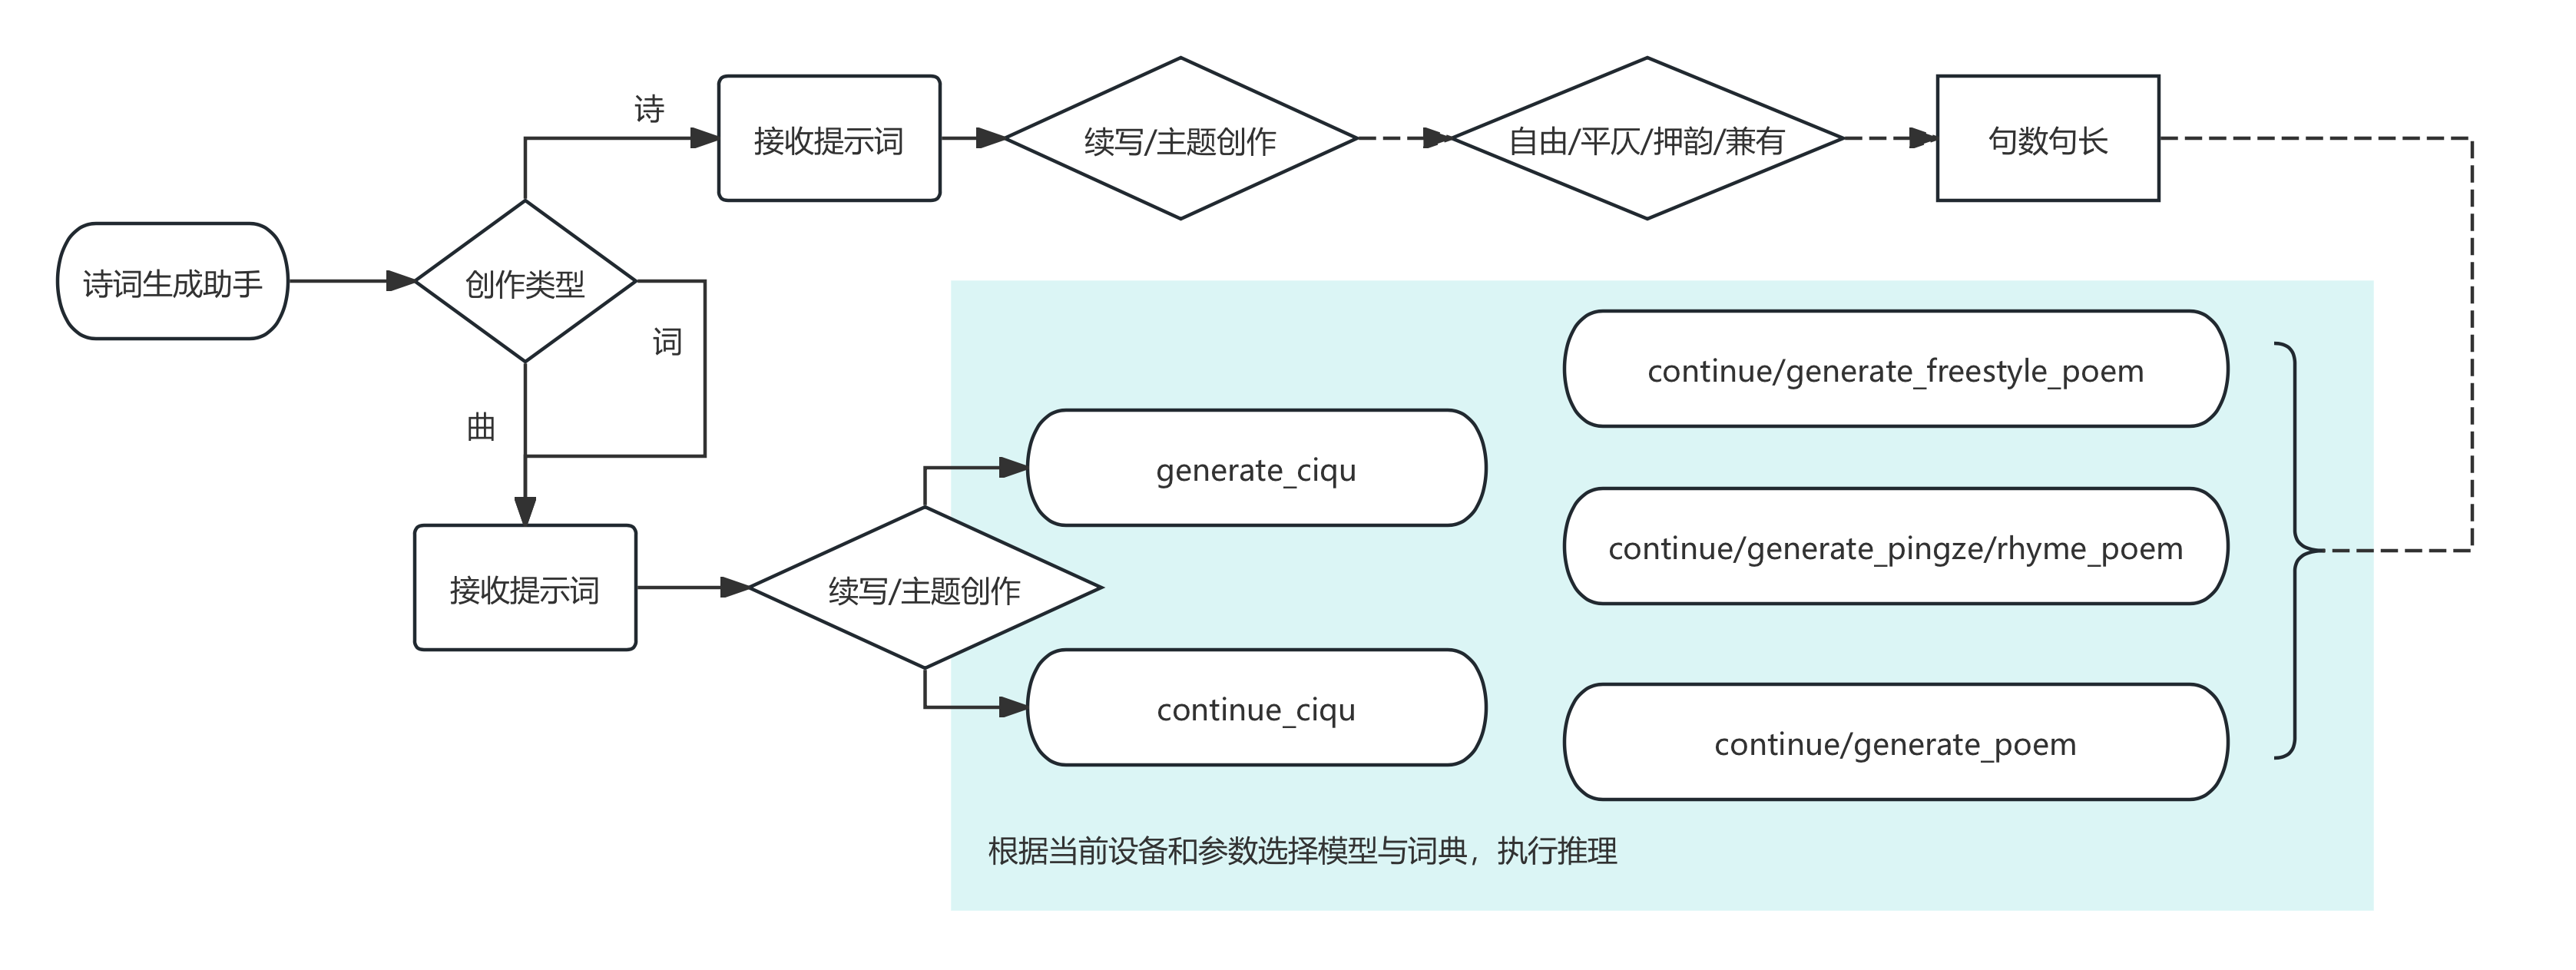
\includegraphics[width=\textwidth]{img/writer/诗词生成助手流程.png}
    \caption{诗词生成助手外部流程示意图}
    \label{fig:iwslt-wmt3}
\end{figure}

\subsection{实现效果}
\textbf{操作台执行结果}
\begin{figure}[h]
    \centering
    % 第一个图像
    \begin{minipage}[b]{0.44\textwidth}
        \centering
        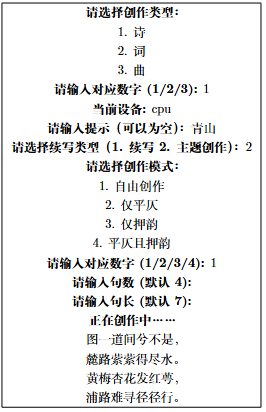
\includegraphics[width=\textwidth]{img/writer/操作台执行结果.png}
        \caption{操作台执行结果}
        \label{fig:operation_result}
    \end{minipage}
    \hfill
    % 第二个图像
    \begin{minipage}[b]{0.49\textwidth}
        \centering
        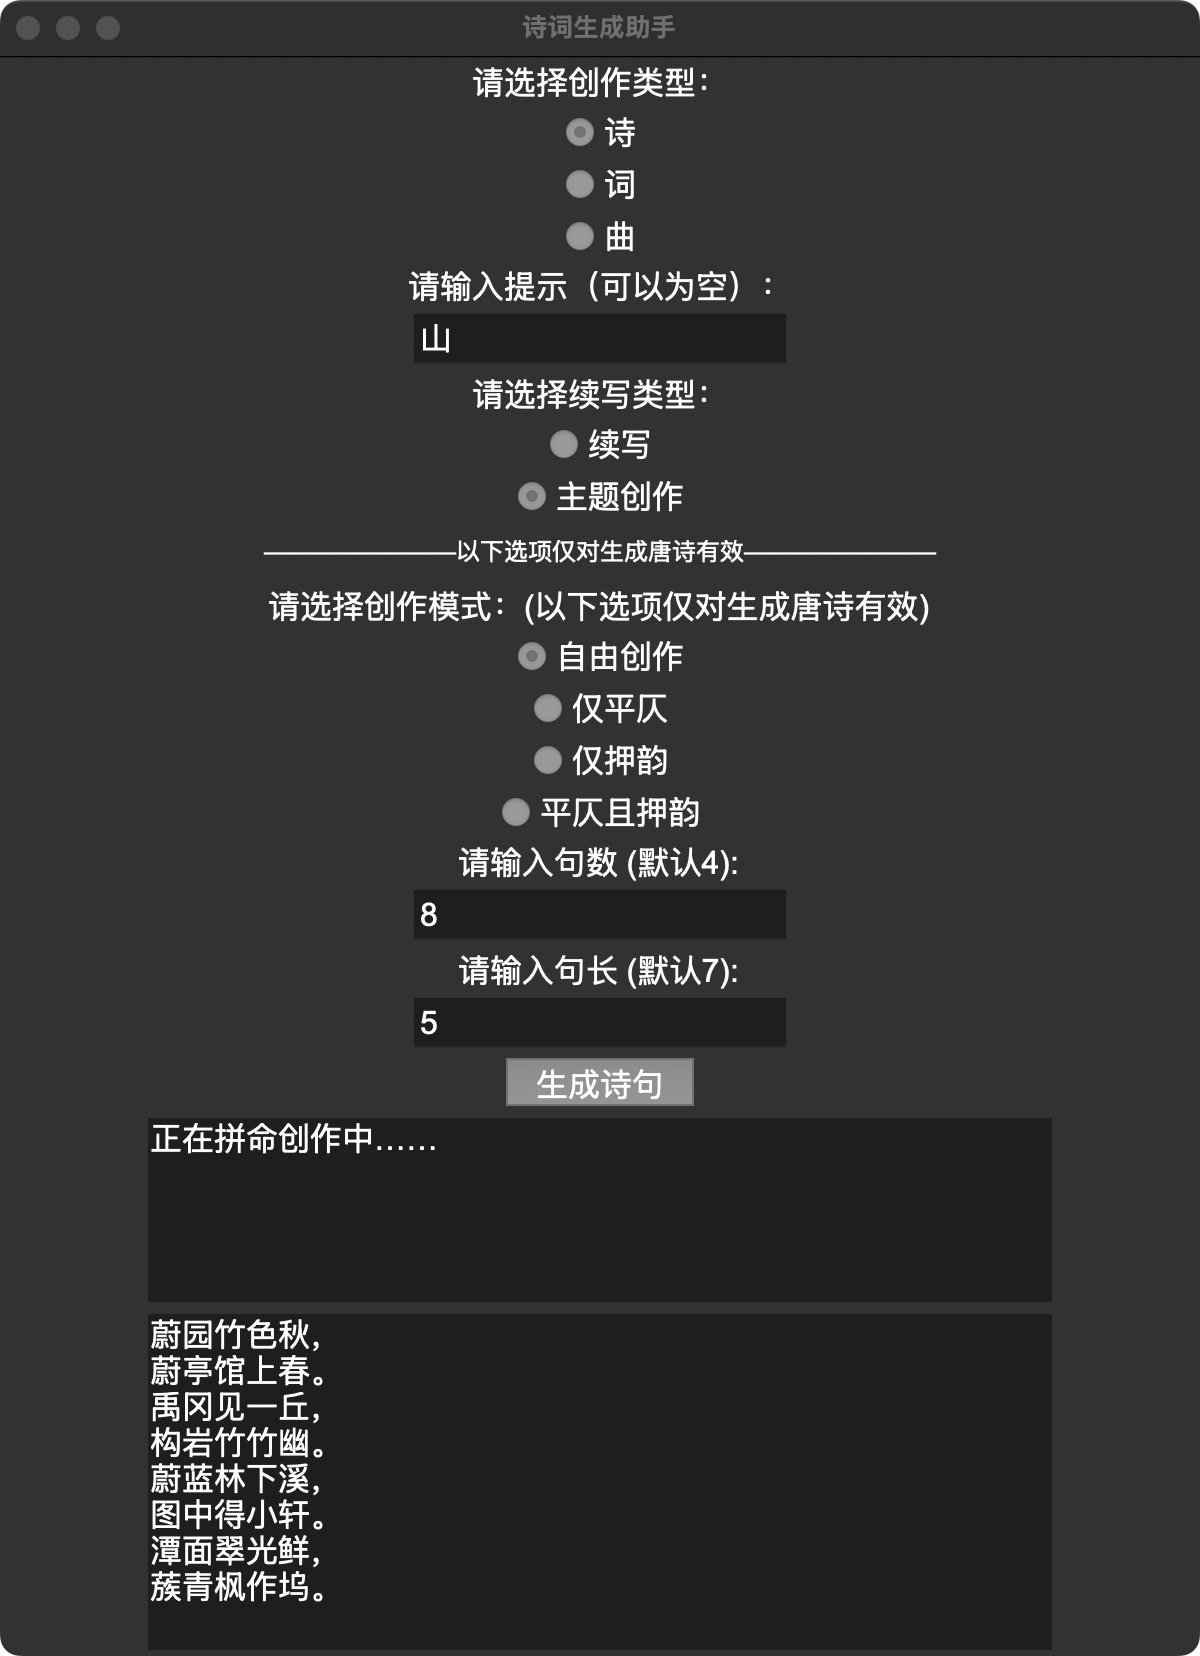
\includegraphics[width=\textwidth]{img/writer/结果1.jpg}
        \caption{诗词生成助手运行展示}
        \label{fig:poem_generator_demo}
    \end{minipage}
\end{figure}

% \section{总结与反思}
\section{总结与反思}\label{sec-8}

\paragraph{丁玺博} 我在本项目中主要负责两篇文献阅读和模型的落地实现部分,整体来说基本完成全部目标。这个过程并不顺利,主要困难是集中在模型的封装调用和改进文本生成逻辑两部分。我清楚认识到一个模型从基本的训练完成到可以自由使用,再到根据实际需求针对性改造与使用,实际上是两个非常艰难、漫长和复杂的过程。特别是结合现实需求的设计,我需要不断去考虑一切可能影响到文本生成的因素,比如模型词向量嵌入步长,src和tgt的动态变化,推理模式随机性的控制等等,并尝试与实际生成古诗文的需求结合起来,比如平仄和韵律。这实在是对一个人耐心和逻辑的极大挑战。如果简单将模型的训练和生成作为后端,用户使用作为前端,那么我确实是对前后端融合以及前端的工作有了更深的认识,这些都是之前仅仅关注模型训练的我所不曾掌握的知识。未来的学习和工作中,我也会更多考虑现实需求和框架融合,而不仅仅关注模型的进步。这学期学习到了非常多有关深度学习的知识,并在手动执行后有了更多的体悟。感谢老师和助教的辛苦付出,遥祝新年快乐,一切顺利。

\paragraph{李健宁} 我在本项目中主要负责精度Transformer原始论文,并仅利用Pytorch基础模块和线性层搭建了自己的Transformer架构。由于之前几乎没有使用Pytorch的经验,在刚开始接触这一部分时第六次作业带给我很大启发。从一开始不清楚初始化和前向传播函数,到能自己完全写出一个模块,在编程过程中进一步感受到了类在编程中的重要作用。在一步一步实现Transformer的过程中,不仅对Transformer的细节有了更加深刻的理解,也对Pytorch中的并行算子。批处理、损失函数等有了更为详细的认知。

代码和算法能力只有在实操中才能得到飞跃,在未来的学习中,我会尝试更多的利用机器学习和深度学习,注重模型的细节和不同模型间的联系,将理论所学与实际操作相结合起来。最后,感谢老师和助教的辛苦付出,让我能深切感受到深度学习的魅力和价值。

\paragraph{肖庆成} 在本项目中,我的主要职责涵盖了两篇关键文献的精读、现有工作的调研、数据集预处理以及将创新性改进应用于自建的Transformer模型。尽管整个过程复杂多变,但总体进展顺利。其中最具有挑战性的环节是将定制化的改进措施融入到手动实现的Transformer架构中,这要求我克服与Python库内置Transformer模型之间的变量命名和函数差异的问题。经过细致的对比和调整,最终成功实现了这一目标。

对于未来的工作,我认为可以在数据集预处理阶段投入更多精力,以期通过引入更丰富的数据资源来进一步优化模型性能。此外,我还意识到,在今后的学习和职业发展中,应更加注重实际应用场景的需求以及不同技术框架间的兼容性,而不仅仅是追求模型算法上的突破。这个学期里,我不仅深入学习了深度学习领域的广泛知识,而且通过实践操作加深了对这些理论的理解。感谢老师和助教团队在整个学期中的悉心指导和支持,祝您们新年快乐,万事如意!


% \section{附表}
\appendix
\section{附表}\label{sec-9}
\begin{table}[h]
    \centering
    \begin{tabular}{l|cc}
    \toprule
    \textbf{Training Steps} & \textbf{65,536} & \textbf{524,288} \\
    \midrule
    $\text{FFN}_{\text{ReLU}}$ (baseline) & 1.997 (0.005) & 1.677 \\
    $\text{FFN}_{\text{GELU}}$ & 1.983 (0.005) & 1.679 \\
    $\text{FFN}_{\text{Swish}}$ & 1.994 (0.003) & 1.683 \\
    \midrule
    $\text{FFN}_{\text{GLU}}$ & 1.982 (0.006) & 1.663 \\
    $\text{FFN}_{\text{Bilinear}}$ & 1.960 (0.005) & 1.648 \\
    $\text{FFN}_{\text{GEGLU}}$ & \textbf{1.942} (0.004) & \textbf{1.633} \\
    $\text{FFN}_{\text{SwiGLU}}$ & \textbf{1.944} (0.010) & \textbf{1.636} \\
    $\text{FFN}_{\text{ReGLU}}$ & 1.953 (0.003) & 1.645 \\
    \bottomrule
\end{tabular}
\caption{Training Setup V.S. log-perplexity}
\label{tab:results}
\end{table}

\begin{table}[ht]
    	\centering
    	\resizebox{\textwidth}{!}{% Adjust the table to fit the text width
    		\begin{tabular}{l|c|cccccccccccc}
    			\toprule
    			& Score & CoLA & SST-2 & MRPC & MRPC & STSB & STSB & QQP & QQP & MNLI & MNLI & QNLI & RTE \\
    			& Average & MCC & Acc & F1 & Acc & PCC & SCC & F1 & Acc & m & mm & Acc & Acc \\
    			\midrule
    			FFN$_{\text{ReLU}}$ & 83.80 & 51.32 & 94.04 & \textbf{93.08} & \textbf{90.20} & 89.64 & 89.42 & 80.01 & 91.75 & 85.83 & 86.42 & 92.81 & 80.14 \\
    			FFN$_{\text{GELU}}$ & 83.86 & 53.48 & 94.04 & 92.81 & \textbf{90.20} & 89.69 & 89.49 & 88.63 & 91.62 & 85.89 & 86.13 & 92.39 & 80.51 \\
    			FFN$_{\text{Swish}}$ & 83.60 & 49.79 & 93.69 & 92.31 & 89.46 & 89.88 & 88.84 & 88.84 & 91.67 & 85.22 & 85.02 & 92.33 & 81.23 \\
    			\midrule
    			FFN$_{\text{GLU}}$ & 84.20 & 49.16 & 94.27 & 92.39 & 89.46 & 89.46 & 89.35 & 88.79 & 91.62 & 86.36 & 86.18 & 92.92 & \textbf{84.12} \\
    			FFN$_{\text{GEGLU}}$ & 84.12 & 53.65 & 93.92 & 92.68 & 89.71 & 90.26 & 90.13 & 89.11 & 91.85 & 86.15 & 86.17 & 92.81 & 79.42 \\
    			FFN$_{\text{BiLinear}}$ & 83.79 & 51.02 & \textbf{94.28} & 92.28 & 89.46 & 90.06 & 89.84 & 88.95 & 91.69 & \textbf{86.90} & \textbf{87.08} & 92.92 & 81.95 \\
    			FFN$_{\text{SwiGLU}}$ & 84.36 & 51.59 & 93.92 & 92.23 & 88.97 & \textbf{90.32} & \textbf{90.13} & \textbf{89.14} & \textbf{89.17} & 86.45 & \textbf{87.47} & \textbf{92.93} & 83.39 \\
    			FFN$_{\text{ReGLU}}$ & \textbf{84.67} & \textbf{56.16} & \textbf{94.28} & 92.06 & 89.22 & 89.97 & 89.85 & 88.86 & 91.72 & 86.20 & 86.40 & 92.68 & 81.59 \\
    			\midrule
    			Raffel et al., 2019 & 83.28 & 53.84 & 92.68 & 92.07 & 88.92 & 88.02 & 87.94 & 88.67 & 91.56 & 84.24 & 84.57 & 90.48 & 76.28 \\
    			ibid. stddev. & 0.235 & 1.111 & 0.569 & 0.729 & 1.019 & 0.374 & 0.418 & 0.108 & 0.070 & 0.291 & 0.231 & 0.361 & 1.393 \\
    			\bottomrule
    	\end{tabular}}
    	\caption{GLUE在语言理解任务上的结果}
    	\label{tab:glue_results1}
\end{table}

\begin{table}[ht]
    \centering
    	\resizebox{\textwidth}{!}{% Adjust the table to fit the text width
    		\begin{tabular}{l|c|ccccccccccc}
    			\toprule
    			& Score & BoolQ & CB & CB & CoPA & MultiRC & MultiRC & ReCoRD & ReCoRD & RTE & WiC & WSC \\
    			& Average & Acc & F1 & Acc & Acc & F1 & EM & F1 & EM & Acc & Acc & Acc \\
    			\midrule
    			$\text{FFN}_{\text{ReLU}}$ (baseline) & 72.76 & 80.15 & 83.37 & 89.29 & 70.00 & 76.39 & 39.14 & 73.73 & 72.91 & 83.39 & 67.71 & 77.88 \\
    			$\text{FFN}_{\text{GELU}}$ & 72.98 & 80.64 & 86.24 & \textbf{91.07} & 74.00 & 75.93 & 38.61 & 72.66 & 72.03 & 81.59 & 68.34 & 75.96 \\
    			$\text{FFN}_{\text{Swish}}$ & 72.40 & 80.43 & 77.75 & 83.93 & 67.00 & 76.34 & 39.14 & 73.34 & 72.36 & 81.95 & 68.18 & 81.73 \\
    			\midrule
    			$\text{FFN}_{\text{GLU}}$ & 73.95 & 80.95 & 77.26 & 83.93 & 73.00 & 76.07 & 39.03 & 74.22 & 73.50 & 84.12 & 67.71 & \textbf{87.50} \\
    			$\text{FFN}_{\text{GEGLU}}$ & 73.96 & 81.19 & 82.09 & 87.50 & 72.00 & \textbf{77.43} & \textbf{41.03} & 75.28 & \textbf{74.60} & 83.39 & 67.08 & 83.65 \\
    			$\text{FFN}_{\text{Bilinear}}$ & 73.81 & \textbf{81.53} & 82.49 & 89.29 & \textbf{76.00} & 76.04 & 40.92 & 74.97 & 74.10 & 82.67 & \textbf{69.28} & 78.85 \\
    			$\text{FFN}_{\text{SwiGLU}}$ & \textbf{74.56} & 81.19 & 82.39 & 89.29 & 73.00 & 75.56 & 38.72 & \textbf{75.35} & 74.55 & \textbf{85.20} & 67.24 & 86.54 \\
    			$\text{FFN}_{\text{ReGLU}}$ & 73.66 & 80.89 & \textbf{86.37} & \textbf{91.07} & 67.00 & 75.32 & 40.50 & 75.07 & 74.10 & 84.88 & 68.04 & 78.81 \\
    			\midrule
    			Raffel et al., 2019 & 71.36 & 76.62 & 91.22 & 91.96 & 66.20 & 66.13 & 25.78 & 69.05 & 76.10 & 73.34 & 68.94 & 78.56 \\
    			ibid, stddev. & 0.416 & 0.365 & 3.237 & 2.560 & 2.741 & 0.716 & 1.011 & 0.370 & 0.379 & 1.228 & 0.850 & 2.029 \\
    			\bottomrule
    	\end{tabular}}
    	\caption{基于预训练微调的语言理解任务结果}
    	\label{tab:glue_results2}
    \end{table}

    \begin{table}[ht]
    \centering
    \begin{tabular}{@{}llcc@{}}
    \toprule
    \textbf{Model} & \textbf{Position Information} & \textbf{EN-DE BLEU} & \textbf{EN-FR BLEU} \\ \midrule
	Transformer (base) & Absolute Position Representations & 26.5 & 38.2 \\
	Transformer (base) & Relative Position Representations & \textbf{26.8} & \textbf{38.7} \\ \midrule
	Transformer (big) & Absolute Position Representations & 27.9 & 41.2 \\
	Transformer (big) & Relative Position Representations & \textbf{29.2} & \textbf{41.5} \\ \bottomrule
    \end{tabular}
    \caption{关于WMT 2014英德(EN-DE)和英法(EN-FR)翻译任务的实验结果,使用的是newstest2014测试集.}
    \label{tab:results1}
\end{table}

\begin{table}[ht]
    \centering
    \begin{tabular}{@{}cc@{}}
    \toprule
	$ k $ & EN-DE BLEU \\ \midrule
	0 & 12.5 \\
	1 & 25.5 \\
	2 & 25.8 \\
	4 & 25.9 \\
	16 & 25.8 \\
	64 & 25.9 \\
	256 & 25.8 \\ \bottomrule
    \end{tabular}
    \caption{关于变化裁剪距离 $ k $的实验结果.}
    \label{tab:clipping-distance-results}
\end{table}

\begin{table}[ht]
    \centering
    \begin{tabular}{@{}ccc@{}}
    \toprule
        $ a_{ij}^V $ & $ a_{ij}^K $ & EN-DE BLEU \\ \midrule
	Yes & Yes & 25.8 \\
	No & Yes & 25.8 \\
	Yes & No & 25.3 \\
	No & No & 12.5 \\ \bottomrule
    \end{tabular}
    \caption{关于相对位置编码 $ a_{ij}^V $和$ a_{ij}^K $的实验结果.}
    \label{tab:ablation-results}
\end{table}

\begin{table}[h]
\centering
\begin{tabular}{|l|c|}
\hline
\textbf{Model} & \textbf{Bits per byte} \\ \hline
\multicolumn{2}{|c|}{\textbf{CIFAR-10}} \\ \hline
PixelCNN (Oord et al., 2016) & 3.03 \\ \hline
PixelCNN++ (Salimans et al., 2017) & 2.92 \\ \hline
Image Transformer (Parmar et al., 2018) & 2.90 \\ \hline
PixelSNAIL (Chen et al., 2017) & 2.85 \\ \hline
Sparse Transformer 59M (strided) & 2.80 \\ \hline
\multicolumn{2}{|c|}{\textbf{Enwik8}} \\ \hline
Deeper Self-Attention (Al-Rfou et al., 2018) & 1.06 \\ \hline
Transformer-XL 88M (Dai et al., 2018) & 1.03 \\ \hline
Transformer-XL 277M (Dai et al., 2018) & 0.99 \\ \hline
Sparse Transformer 95M (fixed) & 0.99 \\ \hline
\multicolumn{2}{|c|}{\textbf{ImageNet 64x64}} \\ \hline
PixelCNN (Oord et al., 2016) & 3.57 \\ \hline
Parallel Multiscale (Reed et al., 2017) & 3.7 \\ \hline
Glow (Kingma \& Dhariwal, 2018) & 3.81 \\ \hline
SPN 150M (Menick \& Kalchbrenner, 2018) & 3.52 \\ \hline
Sparse Transformer 152M (strided) & 3.44 \\ \hline
\multicolumn{2}{|c|}{\textbf{Classical music, 5 seconds at 12 kHz}} \\ \hline
Sparse Transformer 152M (strided) & 1.97 \\ \hline
\end{tabular}
\caption{我们对于密度建模任务的发现总结如下。结果以每字节比特数报告,这等同于图像任务中的每维度比特数。M指的是参数的数量,以百万为单位。}
\label{tab:performance_comparison}
\end{table}

\begin{table}[h]
\centering
\begin{tabular}{|l|c|c|}
\hline
\textbf{Model} & \textbf{Bits per byte} & \textbf{Time/Iter} \\ \hline
\multicolumn{3}{|c|}{\textbf{Enwik8 (12,288 context)}} \\ \hline
Dense Attention & 1.00 & 1.31 \\ \hline
Sparse Transformer (Fixed) & \textbf{0.99} & 0.55 \\ \hline
Sparse Transformer (Strided) & 1.13 & 0.35 \\ \hline
\multicolumn{3}{|c|}{\textbf{CIFAR-10 (3,072 context)}} \\ \hline
Dense Attention & 2.82 & 0.54 \\ \hline
Sparse Transformer (Fixed) & 2.85 & 0.47 \\ \hline
Sparse Transformer (Strided) & \textbf{2.80} & 0.38 \\ \hline
\end{tabular}
\caption{稀疏模式展示了在我们能够比较两者的数据集上,不仅速度得到了提升,而且损失函数值也更优。这可能指向了我们学习到的模式中存在有用的归纳偏置,或者表明全注意力机制下存在潜在的优化问题。}
\label{tab:model_comparison}
\end{table}

\clearpage
\bibliography{ref}
\end{document}

